%\startchapter{Improved Least-Squares Methods for Source Localization: An Iterative Re-Weighting Approach}
\startchapter{Iterative Re-Weighting Least-Squares Methods for Source Localization}
\label{chapter:irw}

Locating a radiating source from range or range-difference measurements in a passive sensor network has recently attracted an increasing amount of research interest as it finds applications in a wide range of network-based wireless systems. Among the useful localization methods that have been documented over the years, least squares based algorithms constitute an important class of solution techniques as they are geometrically meaningful and often provide low complexity solution procedures with competitive estimation accuracy \cite{SmithAbel} - \cite{BeckStLi}. On the other hand, the error measure in a least squares (LS) formulation for the localization problem of interest is shown to be highly nonconvex, possessing multiple local solutions with degraded performance.  There are many methods for continuous unconstrained optimization \cite{AntonLu}, however most of them are \textit{local} methods that are
%iterative, hence extremely 
 sensitive to where the iteration begins, and give no guarantee to yield global solutions when applied to non-convex objective functions. In the case of source localization, this inherent feature of local methods is particular problematic because the source location is assumed to be entirely unknown and can appear practically anywhere, thus the chances to secure a good initial point for a local algorithm are next to none. For these reasons, various ``global'' localization techniques were investigated that are either non-iterative or insensitive to initial iterate. One representative in the class of global localization methods is the convex-relaxation based algorithm for range measurements proposed in \cite{Cheung}, where the least squares model is relaxed to a semidefinite programming problem which is known to be convex \cite{VBoyd}, hence robust to where it starts. Another representative in this class is reference \cite{BeckStLi}, where localization problems for  range as well as range difference measurements are addressed by developing solution methods for \textit{squared} range LS (SR-LS) and \textit{squared} range difference LS (SRD-LS) problems. The methods proposed in \cite{BeckStLi} are non-iterative and the solutions obtained are proven to be the global minimizers of the respective SR-LS and SRD-LS problems, which are shown to be excellent estimates of the original LS solutions.

This chapter presents improved least squares methods that demonstrate improved localization performance when compared with some best known results from the literature. The key new ingredient of the proposed algorithms is an iterative procedure where the SR-LS (SRD-LS) algorithm is iteratively applied to a weighted sum of squared terms where the weights are carefully designed so that the iterates produced quickly converge to a solution which is found to be considerably closer to the original range-based (range-difference-based) LS solution. % that is known to be the maximum-likelihood estimator in the case of Gaussian white measurement noise. Numerical results are presented for performance evaluation and comparisons.



\section{Source Localization Using Range Measurements}%II
\subsection{Problem Statement}%2.1


The source localization problem considered here involves a given array of $m$ sensors specified by $\{\Ba_1,\ldots, \Ba_m\}$ where $\Ba_i\in R^n$  contains the $n$ coordinates of the $i$th sensor in space $R^n$. Each sensor measures its distance to a radiating source $\Bx\in R^n$. Throughout it is assumed that only noisy copies of the distance data are available, hence the \textit{range measurements} obey the model
\begin{equation} \label{eq:3.1}
\setcounter{equation}{1}
r_i = \|{\Bx} - {\Ba}_i\| + \varepsilon_i, i = 1,\ldots , m.
\end{equation}                                                                                                     	where $\varepsilon_i$ denotes the unknown noise that has occurred when the $i$th sensor measures its distance to source $\Bx$. Let $\Br=[r_1 \ r_2 \ldots r_m]^T$ and $\Beps=[\varepsilon_1 \ \varepsilon_2 \ldots \varepsilon_m]^T$. The source localization problem can be stated as to estimate the exact source location $\Bx$ from the noisy range measurements $\Br$. In the rest of this section, a least-squares (LS) formulation of the localization problem and two most relevant state-of-the-art solution methods are briefly reviewed; and a new method based on iterative re-weighting of squared range LS technique as well as a variant of the proposed method are then presented. %; and numerical results for performance evaluation and comparisons of the relevant algorithms are reported.

%
%The source localization problem considered here involves a given array of $m$ sensors specified by $\{\Ba_1,\ldots, \Ba_m\}$ where $\Ba_i\in R^n$  contains the $n$ coordinates of the $i$th sensor in space $R^n$. Each sensor measures its distance to a radiating source $\Bx\in R^n$. Throughout it is assumed that only noisy copies of the distance data are available, hence the \textit{range measurements} obey the model
%\begin{equation} \label{eq:3.0}
%\setcounter{equation}{1}
%r_i = \|{\Bx} - {\Ba}_i\| + \varepsilon_i, i = 1,\ldots , m.
%\end{equation}                                                                                                     	where $\varepsilon_i$ denotes the unknown noise that has occurred when the $i$th sensor measures its distance to source $\Bx$. Let $\Br=[r_1 \ r_2 \ldots r_m]^T$ and $\Beps=[\varepsilon_1 \ \varepsilon_2 \ldots \varepsilon_m]^T$. The source localization problem can be stated as to estimate the exact source location $\Bx$ from the noisy range measurements $\Br$. 
%
%For the localization problem at hand, the range-based least squares (R-LS) estimate refers to the solution of the problem
%\begin{equation}\label{eq:3.1} %eq 2
%\Min_{\Bx} \quad F(\Bx)=\sum_{i=1}^{m} (r_i - \|{\Bx} - {\Ba}_i\|)^2
%\end{equation}
%
%Formulation (\ref{eq:3.2}) is connected to the maximum-likelihood (ML) location estimation that determines $\Bx$ by examining the probabilistic model of the error vector $\Beps$. If $\Beps$ obeys a Gaussian distribution with zero mean and covariance $\symb{\Sigma} = \mbox{diag}(\sigma_1^2, \ldots, \sigma_m^2)$, then the maximum likelihood (ML) location estimator in this case is known to be
%\begin{equation} \label{eq:3.3}%eq 3
%\Bx_{ML} = \mbox{arg}\!\min_{{\Bx} \in R^n} (\Br - \Bg)^T\Sigma^{-1}(\Br - \Bg)
%\end{equation}
%where $\Bg = [g_1 \ g_2 \ldots \ g_m]^T$ with $g_i = \|{\Bx} - {\Ba}_i\|$. It follows immediately that the ML solution in (\ref{eq:3.3}) is identical to the R-LS solution of problem (\ref{eq:3.2}) when covariance $\symb{\Sigma}$ is proportional to the identity matrix, i.e., $\sigma_1^2=\ldots =\sigma_m^2 = 1$. In the literature this is known as the equal noise power case. For notation the method described in this chapter focuses on the equal noise power case, however the method developed below is also applicable to the unequal noise power case by working on a weighted version of the objective in  (\ref{eq:3.2})  with $\{\sigma_i^{-2}, i = 1, \ldots, m\}$ as the weights.
%
%
%In the rest of this section, a least-squares (LS) formulation of the localization problem and two most relevant state-of-the-art solution methods are briefly reviewed; and a new method based on iterative re-weighting of squared range LS technique as well as a variant of the proposed method are then presented.

\subsection{LS Formulations and Review of Related Work} %2.2

Least squares approaches have proven effective for source localization problems \cite{SmithAbel} -\cite{BeckStLi}. For the localization problem at hand, the range-based least squares (R-LS) estimate refers to the solution of the problem
\begin{equation}\label{eq:3.2} %eq 2
%(R-LS): \Min_{\Bx} \sum_{i=1}^{m} (r_i - \|{\Bx} - {\Ba}_i\|)^2
\Min_{\Bx} f(\Bx) \equiv \sum_{i=1}^{m} (r_i - \|{\Bx} - {\Ba}_i\|)^2
\end{equation}

%\{As could be seen the problem (\ref{eq:3.2}) at hand is nonconvex [].\}
The primary reason that justifies formulation (\ref{eq:3.2}) is its connection to the maximum-likelihood location estimation that determines $\Bx$ by examining the probabilistic model of the error vector $\Beps$. Assuming the errors $\varepsilon_i$ are independent and identically distributed (i.i.d.) Gaussian variables with zero mean and variance $\sigma_i^2$, then $\Beps$ obeys a Gaussian distribution with zero mean and covariance $\symb{\Sigma} = \mbox{diag}(\sigma_1^2, \ldots, \sigma_m^2)$, and the maximum likelihood (ML) location estimator in this case is known to be
\begin{equation} \label{eq:3.3}%eq 3
\Bx_{ML} = \mbox{arg}\!\min_{{\Bx} \in R^n} (\Br - \Bg)^T\Sigma^{-1}(\Br - \Bg)
\end{equation}
where $\Bg = [g_1 \ g_2 \ldots \ g_m]^T$ with
\begin{equation} \label{eq:3.4}%eq 4
g_i = \|{\Bx} - {\Ba}_i\|
\end{equation}
It follows immediately that the ML solution in (\ref{eq:3.3}) is identical to the R-LS solution of problem (\ref{eq:3.2}) when covariance $\symb{\Sigma}$ is proportional to the identity matrix, i.e., $\sigma_1^2=\ldots =\sigma_m^2$. In the literature this is known as the equal noise power case. For notation simplicity the method described in this chapter focuses on the equal noise power case, however the method developed below is also applicable to the unequal noise power case by working on a weighted version of the objective in  (\ref{eq:3.2})  with $\{\sigma_i^{-2}, i = 1, \ldots, m\}$ as the weights.

Although many methods for unconstrained optimization are available \cite{AntonLu}, most of them are \textit{local} methods in the sense they are sensitive to the choice of initial point where the iteration of an optimization algorithm begins. Especially when applied to a nonconvex objective function which possesses a number of local minimizers, unless a chosen local method starts at an initial point that happens to be sufficiently close to the (unknown) global minimizer, the solution obtained by the method gives no guaranty about global minimality. Unfortunately, the objective in (\ref{eq:3.2}) is highly nonconvex, possessing many local minimizers even for small-scale systems. As an example, consider an instance of the source localization problem on the plane $n = 2$ with five sensors $ m = 5$ located at $(6,4)^T, (0,-10)^T, (5,-3)^T, (1,-4)^T$ and  $(3,-3)^T$ with the source emmitting the signal at $\Bx_s = (-2,3)^T$. Figure \ref{fig:ExampleOfRLSNonconvexity} depicts a contour plot of the R-LS objective function in (\ref{eq:3.2}) over the region $\Re = \{\Bx: -6 \leq x_1 \leq 13, -10 \leq x_2 \leq 9 \}$. It can be observed from the plot that there are two minimizers at $\tilde{\Bx} = (-1.9907, 3.0474)^T$ and $\widehat{\Bx} = (11.1152, -2.6785)^T$ with values of the objective  $f(\tilde{\Bx}) = 0.1048 $ and $f(\widehat{\Bx}) = 15.0083$ respectively. As expected, the global minimizer of R-LS objective offers a good approximation of the exact source location $\Bx_s$, but is unlikely to be precisely at point $\Bx_s$ because the objective $f(\Bx)$ is defined using noisy range measurements. Note that for the exact source location $\Bx_s$ we have $f(\Bx_s) = \sum_{i=1}^m \varepsilon_i^2$.

\begin{figure*}[t]
\centering
  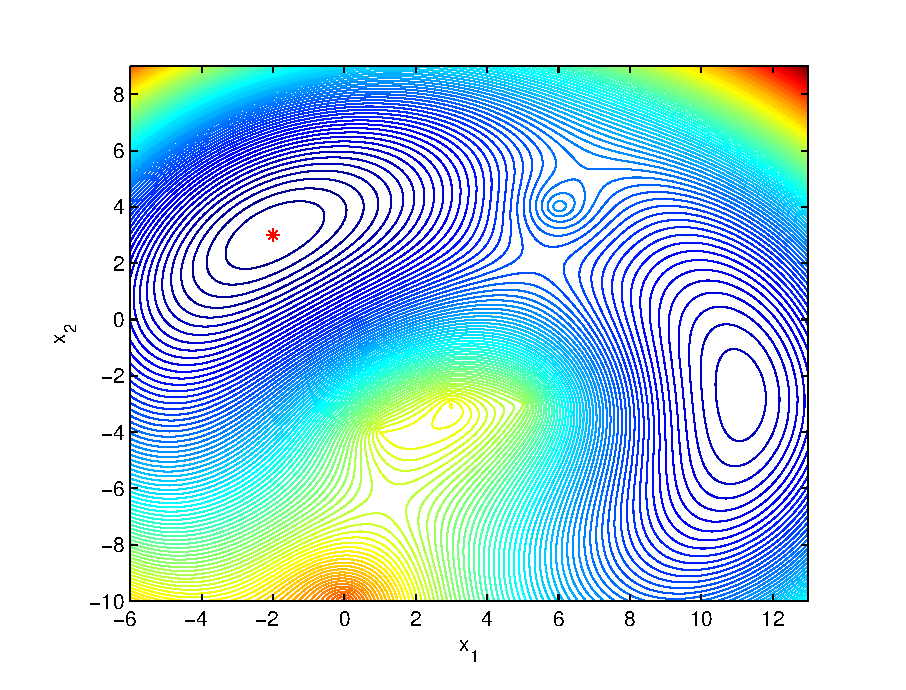
\includegraphics{figures/nonconvexity_example_ls_new_range}
\caption{Contours of the R-LS objective function over the region $\protect\Re = \protect\lbrace \protect\Bx:-6\protect\leq x_1 \protect\leq 13, -10\protect\leq x_2 \protect\leq 9 \protect\rbrace$}
\label{fig:ExampleOfRLSNonconvexity}
\end{figure*}

Reference \cite{Cheung} addresses problem (\ref{eq:3.2}) by a convex relaxation technique where (\ref{eq:3.2}) is modified to a convex problem known as semidefinite programming (SDP) \cite{VBoyd}. A key step in this procedure is to use (\ref{eq:3.4}) with  $g_i$ as new variables, which leads (\ref{eq:3.2}) to the constrained problem
\begin{eqnarray} \label{eq:3.5}%eq 5 a,b
\setcounter{abc}{1}
\Min_{{\Bx}, {\Bg}} \sum_{i=1}^m (r_i - g_i)^2\qquad\\
\stepcounter{abc} \setcounter{equation}{5} 
\mbox{subject to: \ } g_i^2=\|{\Bx} - {\Ba_i}\|^2,\quad i = 1, \ldots,m.
\end{eqnarray}
By further defining matrix variables
\begin{equation} \label{eq:3.6}%eq 6
\setcounter{abc}{0}
\BG = \left[\begin{array}{c} \Bg \\
1 \end{array}\right] \left[ \begin{array}{cc} \Bg^T & 1 \end{array} \right] \mbox{and } \BX = \left[\begin{array}{c} \Bx \\
1 \end{array}\right] \left[ \begin{array}{cc} \Bx^T & 1 \end{array} \right]
\end{equation}
and neglecting the rank constrains on $\BG$ and $\BX$, (\ref{eq:3.5}) can be reformulated in term of variables $\BG$ and $\BX$ as
\begin{eqnarray}
\setcounter{abc}{0}
\label{eq:3.7}
\setcounter{abc}{0} % before was 12, now change to 7 - WSLU
\setcounter{abc}{1}\setcounter{equation}{7}
\Min_{\BX,\BG} \sum_{i=1}^{m} \left(G_{ii}- 2r_iG_{m+1,i}+r_i^2\right)\qquad\\
\stepcounter{abc}\setcounter{equation}{7}
\mbox{subject to: \ } G_{ii}=\boldmath{Tr}\left(\BC_i\BX\right), i = 1, \ldots,m \\
\stepcounter{abc}\setcounter{equation}{7}
\BG \succeq 0, \BX \succeq 0 \quad\qquad\qquad\qquad\\
\stepcounter{abc}\setcounter{equation}{7}
G_{m+1,m+1}=G_{n+1,n+1}=1 \quad
\end{eqnarray}
where
\begin{equation} \label{eq:3.8} % put here as 8
\setcounter{abc}{0}
\setcounter{equation}{8}
C_i=\left( \begin{array}{cc}  \BI\!_{n\times n} & -\Ba_i
\\ -\Ba_i^T & \|\Ba_i\|^2 \\
\end{array}\right) \quad i=1,\ldots,m
\end{equation}
which is a standard SDP problem that can be solved efficiently \cite{VBoyd,AntonLu}. Note that because (\ref{eq:3.7}) is a convex problem, global minimality of the solution is ensured regardless of the initial point used. On the other hand, however, because (\ref{eq:3.7}) is an approximation of the original problem in (\ref{eq:3.2}), the solution of (\ref{eq:3.7}) is only an approximate solution of problem (\ref{eq:3.2}). In what follows the solutions obtained by this SDP-relaxation based method will be referred to as SDR-LS solutions.

A rather different approach is recently proposed in \cite{BeckStLi} where the localization problem (\ref{eq:3.2}) is tackled by developing techniques that find global solution of the \textit{squared range based LS} (SR-LS) problem
\begin{equation} \label{eq:3.9}%eq 9
\Min_{\Bx} \sum_{i=1}^{m} \left(\|{\Bx} - {\Ba}_i\|^2 - r_i^2\right)^2
\end{equation}
By writing the objective in (\ref{eq:3.9}) as $\left(\alpha-2\Ba_i^T\Bx+\|\Ba_i\|^2-r_i^2\right)^2$ with $\alpha=\|\Bx\|^2$, it becomes a convex quadratic objective if one treats $\alpha$  as an additional variable and  $\alpha=\|\Bx\|^2$  as a constraint. In this way, (\ref{eq:3.9}) is converted to the following constrained LS problem after necessary variable changes:
\begin{eqnarray} \label{eq:3.10}
\setcounter{abc}{1}
\Min_{{\By} \in R^{n+1}} \|\BA\By-\Bb\|^2 \qquad\\
\stepcounter{abc} \setcounter{equation}{10} \mbox{subject to: \ }
\By^T\BD\By + 2\Bf^T\By = 0
\end{eqnarray}
where
\setcounter{abc}{0}
\begin{equation} \label{eq:3.11}
\setcounter{abc}{0}
\setcounter{equation}{11}
\By = \left(\begin{array}{c}
\Bx \\
\|\Bx\|^2 
\end{array} \right), \;
\BA=\left(\begin{array}{cc}
    -2\Ba_1^T & 1 \\
    \vdots  & \vdots \\
    -2\Ba_m^T & 1
    \end{array} \right), \;
\Bb=\left(\begin{array}{c}
    r_1^2-\|\Ba_1\|^2 \\
    \vdots \\
    r_m^2-\|\Ba_m\|^2
    \end{array} \right)
\end{equation}
\begin{equation}% \label{eq:3.12}
\nonumber
\BD=\left(\begin{array}{cc}
    \BI\!_{n\times n} & \BO_{n\times n} \\
    \BO_{n\times n} & 0
    \end{array} \right), \;
\Bf=\left(\begin{array}{c}\BO \\ -0.5 \end{array} \right)
\end{equation}
This problem conversion, made in \cite{BeckStLi}, turns out to be crucial as problem (\ref{eq:3.10}), which remains to be nonconvex because of the nonlinear equality constraint (\ref{eq:3.10}b), falls into the class of generalized trust region subproblems (GTRS) \cite{More, FortinWol}  whose global solutions can be computed by exploring the KKT conditions which are both necessary and sufficient optimality conditions in this case \cite{More}.

We now conclude this section with a couple of remarks. First, an unconstrained version of (\ref{eq:3.10}) may be obtained by neglecting the constraint in (\ref{eq:3.10}b) as
\begin{equation} \label{eq:3.12}%eq 13
\Min_{{\By} \in R^{n+1}} \|\BA\By-\Bb\|^2
\end{equation}
whose solution, called \textit{unconstrained squared-range-based LS }(USR-LS) estimate, is given by
\begin{equation} \label{eq:3.13}%eq 14
\By^*=\left(\BA^T\!\BA\right)^{-1}\!\!\!\!\BA^T\Bb
\end{equation}
It is demonstrated by numerical experiments \cite{BeckStLi} that the SR-LS solution outperforms the USR-LS and, in many cases, SDR solutions. Second, the SR-LS solution, although it solves (\ref{eq:3.9}) exactly, lacks the statistical interpretation of the ML formulation. The SR-LS remains to be an approximate solution for the original problem in (\ref{eq:3.2}) and, as it was demonstrated by the numerical results in \cite{BeckTeCh} and \cite{BeckGPS}, provides less accurate estimates of the true source location, than the LS estimate. The method, described in detail below, tries to reduce the gap between the two solutions.

\subsection{An Iterative Re-Weighting Approach}%2.3

%An iterative re-weighting minimization schemes in several forms has been proposed in the literature \cite{BeckTeCh}, \cite{Beck15}. The standard fixed point (SFP) algorithm \cite{BeckTeCh} was constructed similarly to the Weizfeld method that was designed to solve the Fermat-Weber problem. The iterates of SPF were constructed from the optimality conditions for (\ref{eq:3.2}). SPF is a gradient method with a fixed step size. Proposed schemes for choosing the initial point $\Bx_0$ guarantees the convergence and eliminates points of non-smoothness
%and the sequential weighted least squares algorithms (SWLS) \cite{BeckTeCh} are based 

Iterative re-weighting least squares method is a popular technique used for solving problems involving the sums of norms. The method has found many applications, such as in robust regression \cite{RReg, GIRLS}, sparse recovery \cite{Daub}, but the most relevand application for the current case is for solving the Fermat-Weber location problem. The Fermat--Weber problem %is one of the oldest easily-stated nontrivial problems in computational geometry: 
has a long history and has been extensively studied in the field of optimization and location theory \cite{GIRLS}. This problem can be stated as: Given $m$ points $\Ba_1, \Ba_2, \ldots, \Ba_m \in R^n$ called \textit{anchors} and nonnegative weights $\omega_1, \omega_2, \ldots, \omega_m > 0$, find $\Bx \in R^n$ that minimizes the weighted sum of Euclidian distances between $\Bx$ and the $m$ anchors:
\begin{equation} \label{eq:FW}
\nonumber
\Min_{\Bx \in R^n} \sum_{i=1}^{m} \omega_i\|\Bx - \Ba_i\|.
\end{equation}
Fermat--Weber problem is much easier to analyze and solve than the ML problem (\ref{eq:3.2}) because it is a well-structured nonsmooth convex minimization problem. 
%However the similarities of these problems has been noted in the literature \cite{BeckTeCh}.
%This problem has a long history and has been extensively studied in the field of optimization and location theory.
%the most famous and oldest example of the IRLS method is Weiszfeld’s method for solving the Fermat–Weber problem — an algorithm that was introduced in 1937.
% Our objective here is to mimic the Weiszfeld algorithm [16] to obtain an algorithm for solving the nonsmooth and nonconvex ML problem (1.2). The Weiszfeld method is a very simple fixed-point scheme that is designed to solve the Fermat–Weber problem. One way to derive it is to write the first order global optimality conditions for the convex problem (2.1)
The similarities between the Fermat--Weber problem and problem (\ref{eq:3.2}) have been noted and addressed in the literature \cite{BeckTeCh} with a gradient method with a fixed step size, known as the standard fixed point (SFP) algorithm, to deal with problem (\ref{eq:3.2}). However, being a gradient method, likelihood for the SFP algorithm to converge to a local solution exists. Another method, also proposed in \cite{BeckTeCh} and known  as the the sequential weighted least squares algorithm (SWLS), is also an iterative method where each iteration involves solving a nonlinear least squares problem similar to (\ref{eq:3.9}). The SWLS method is found to be superior over SFP in terms of convergence rate and a wider region of convergence to the global minimum \cite{BeckTeCh}. However, the possibility for SWLS to converge to a local minimum remains in certain sensor setups even if the initial point is constructed using a procedure developed specifically for SWLS. The method presented below takes an approach that is different from those described above in the sense that it does not require an initial point and the solution produced is guranteed to converge to a \textit{global} solution. 

\subsubsection{Weighted squared range based least squares formulation} %2.3.1

We now consider the weighted squared range based least squares (WSR-LS) problem
\begin{equation} \label{eq:3.14} %eq 15
\Min_{\Bx} \sum_{i=1}^{m} w_i\left(\|{\Bx} - {\Ba}_i\|^2 - r_i^2\right)^2
\end{equation}
which is obviously a weighted version of the SR-LS problem in (\ref{eq:3.9}). Following \cite{BeckStLi}, it is rather straightforward to convert (\ref{eq:3.14}) into a GTRS similar to (\ref{eq:3.10}) as
\begin{eqnarray} \label{eq:3.15} %eq 16 a,b
\setcounter{abc}{1}
\Min_{{\By} \in R^{n+1}} \|\BGA\left(\BA\By-\Bb\right)\|^2 \qquad\\
\stepcounter{abc} \setcounter{equation}{15} \mbox{subject to: \ }
\By^T\BD\By + 2\Bf^T\By = 0
\end{eqnarray}
where $\BA$, $\Bb$, $\BD$, and $\Bf$ are defined in (\ref{eq:3.11}) and $\BGA=\mbox{diag}\left(\sqrt{w_1},\ldots,\sqrt{w_m}\right)$. Clearly, problem (\ref{eq:3.15}) can be written as
\begin{eqnarray}
\setcounter{abc}{0}
\label{eq:3.16}%eq 17 a,b
\setcounter{abc}{1}
\Min_{{\By} \in R^{n+1}} \|\BA_w\By-\Bb_w\|^2 \qquad\\
\stepcounter{abc} \setcounter{equation}{16} \mbox{subject to: \ }
\By^T\BD\By + 2\Bf^T\By = 0
\end{eqnarray}
where $\BA_w = \BGA\BA$ and $\Bb_w=\BGA\Bb$. On comparing (\ref{eq:3.16}) with (\ref{eq:3.10}), %we conclude that 
if $S(\BA,\Bb,\BD,\Bf)$ denotes a solver that produces the global solution of problem (\ref{eq:3.10}) for a given data set $\{\BA,\Bb,\BD,\Bf\}$, then the same solver produces the global solution of the weighted problem (\ref{eq:3.14}) as long as it is applied to the data set $\{\BA_w,\Bb_w,\BD,\Bf\}$. We stress that the weights $\{w_i, i=1,\ldots, m\}$ in (\ref{eq:3.14}) are \textit{fixed} nonnegative constants.


\subsubsection{Moving the SR-LS solution towards R-LS solution via iterative re-weighting}% 2.3.2

The main idea here is to use the weights $\{w_i, i=1,\ldots, m\}$  to tune the objective in (\ref{eq:3.14}) toward the objective in (\ref{eq:3.2}) so that the solution obtained by minimizing such a WSR-LS objective is expected to be closer toward that of the problem (\ref{eq:3.2}). To substantiate the idea, we compare the $i$th term of the objective in (\ref{eq:3.14}) with its counterpart in (\ref{eq:3.2}), namely,
\begin{equation} \label{eq:3.17} %eq 18
\setcounter{abc}{0}
\underbrace{w_i\left(\|\Bx-\Ba_i\|^2-r_i^2\right)^2}_{\mbox{in (15)}}\leftrightarrow\underbrace{\left(\|\Bx-\Ba_i\|-r_i\right)^2}_{\mbox{in (2)}}
\end{equation}
and write the term in (\ref{eq:3.14}) as
\begin{equation} %\label{eq:3.18}%eq19
\nonumber
\begin{array}{l}
w_i\left(\|\Bx-\Ba_i\|^2-r_i^2\right)^2 = \\ w_i\left(\|\Bx-\Ba_i\|+r_i\right)^2 \underbrace{\left(\|\Bx-\Ba_i\|-r_i\right)^2}_{\mbox{same as in (2)}}
\end{array}
\end{equation}
It follows that the objective in (\ref{eq:3.14}) would be the same as in (\ref{eq:3.2}) if the weights $w_i$ were assigned to $1/\left(\|\Bx-\Ba_i\|+r_i\right)^2$. Evidently, weight assignments as such cannot be realized because $w_i$'s must be fixed constants for (\ref{eq:3.14}) to be a globally solvable WSR-LS problem. A natural remedy to deal with this technical difficulty is to employ an iterative procedure whose $k$th iteration generates a global solution $\Bx_k$  of a WSR-LS sub-problem of the form
\begin{equation}\label{eq:3.19}% eq20
\Min_{x} \sum_{i=1}^m w_i^{(k)}\left(\|\Bx-\Ba_i\|^2-r_i^2\right)^2
\end{equation}
where for $k\geq2$ the weights $\{w_i^{(k)},i=1,\ldots,m\}$ are assigned using the previous iterate $\Bx_{k-1}$ as
\begin{equation} \label{eq:3.20}%eq 21
w_i^{(k)}=\frac{1}{\left(\|\Bx_{k-1}-\Ba_i\|+r_i\right)^2}
\end{equation}
while for $k=1$ all weights $\{w_i^{(1)}, i=1,\ldots, m\}$ are set to unity. Clearly the weights given by (\ref{eq:3.20}) are realizable. More importantly, when the iterates produced by solving (\ref{eq:3.19}) (namely $\Bx_k$ for $k = 1, 2,\ldots$) converge, in the $k$th iteration with $k$ sufficiently large, the objective function of (\ref{eq:3.19}) in a small vicinity of its solution $\Bx_k$ is approximately equal to
\begin{equation} \label{sr:w}
\nonumber
\begin{aligned}
&\sum_{i=1}^m w_i^{(k)}\left(\|\Bx-\Ba_i\|^2-r_i^2\right)^2 \\
 \approx &\sum_{i=1}^m w_i^{(k)}\left(\|\Bx_k-\Ba_i\|^2-r_i^2\right)^2 \\
 =&\sum_{i=1}^m w_i^{(k)}\left(\|\Bx_k-\Ba_i\|+r_i\right)^2\left(\|\Bx_k-\Ba_i\|-r_i\right)^2  \\
 \approx &\sum_{i=1}^m w_i^{(k)}\left(\|\Bx_{k-1}-\Ba_i\|+r_i\right)^2\left(\|\Bx_k-\Ba_i\|-r_i\right)^2 \\
 =&\sum_{i=1}^m \left(\|\Bx_k-\Ba_i\|-r_i\right)^2 \approx \sum_{i=1}^m \left(\|\Bx-\Ba_i\|-r_i\right)^2\\
\end{aligned}
\end{equation}
%In other words, after infinite amount of iterations the WSR-LS solution to the problem (\ref{eq:3.19}) is expected to converge to the global solution of problem (\ref{eq:3.2}). [ Would this wording
In words, with the weights from (\ref{eq:3.20}), the limiting point of the iterates produced by iteratively solving WSR-LS problem (\ref{eq:3.19}) is expected to be close to the global solution of problem (\ref{eq:3.2}).

The algorithmic steps of the proposed localization method are outlined as follows.

\phantom{m}
\framebox{%
\parbox{5.5in}{
\noindent \textbf{Algorithm 1} \label{alg:r-ls}

1) Input data: Sensor locations $\{\Ba_i, i=1,\ldots,m\}$, range measurements $\{r_i, i=1,\ldots,m\}$, maximum number of iterations $k_{max}$ and convergence tolerance $\zeta$.

2) Generate data set $\{\BA,\Bb, \Bd, \Bf \}$ as
\begin{equation} 
\nonumber
\BA=\left(\begin{array}{cc}
    -2\Ba_1^T & 1 \\
    \vdots  & \vdots \\
    -2\Ba_m^T & 1
    \end{array} \right),
\Bb=\left(\begin{array}{c}
    r_1^T-\|\Ba_1\|^T \\
    \vdots \\
    r_m^T-\|\Ba_m\|^T
    \end{array} \right)
\end{equation}
\begin{equation} 
\nonumber
\BD=\left(\begin{array}{cc}
    \BI\!_{n\times n} & \BO_{n\times n} \\
    \BO_{n\times n} & 0
    \end{array} \right),
\Bf=\left(\begin{array}{c}\BO \\ -0.5 \end{array} \right) .
\end{equation}

Set $k=1, w_i^{(1)}=1$ for $i=1,\ldots,m$.

3) Set $\BGA_k=\mbox{diag}\left(\sqrt{w_1^{(k)}},\ldots,\sqrt{w_m^{(k)}}\right)$, $\BA_w=\BGA_k\BA$ and $\Bb_w=\BGA_k\Bb$.

4) Solve the WSR-LS problem 
% 3.20
\begin{equation} 
\nonumber 
\Min_{x} \sum_{i=1}^m w_i^{(k)}\left(\|\Bx-\Ba_i\|^2-r_i^2\right)^2
\end{equation}
by solving (\ref{eq:3.16}), i.e.
% 3.21
\begin{equation}
\nonumber
\begin{aligned}
&\Min_{{\By} \in R^{n+1}} \|\BA_w\By-\Bb_w\|^2 \\
&\mbox{subject to: \ }  \By^T\BD\By + 2\Bf^T\By = 0
\end{aligned}
\end{equation} 
to obtain its global solution $\Bx_k$.

5) If $k=k_{max}$ or $\|\Bx_k-\Bx_{k-1}\|<\zeta$, terminate and output $\Bx_k$ as the solution; otherwise, set $k=k+1$, update weights $\{w_i^{(k)}, i=1,\ldots,m\}$ using % 3.21
\begin{equation}
\nonumber
w_i^{(k)}=\frac{1}{\left(\|\Bx_{k-1}-\Ba_i\|+r_i\right)^2}
\end{equation}
and repeat from Step 3).
}
}

\phantom{m}

From the steps in Algorithm 1, it follows that the complexity of the algorithm is practically equal to the complexity of the WSR-LS solver involved in Step 4 times the number of iterations, $k$. Computer simulations have indicated that the algorithm converges with a small number of iterations, typically a $k\leq6$  suffices. For simplicity, the solutions obtained from Algorithm 1 are called IRWSR-LS solutions. Technical details on how to solve (\ref{eq:3.16}) can be found in Appendix 1.

\subsubsection{A variant of Algorithm 1}% 2.3.3

As argued above, the IRWSR-LS solution from Algorithm 1 is expected to be an improved approximation of the global solution of R-LS problem in (\ref{eq:3.2}). However a small gap between the two solutions is inevitable owing to the approximate nature of the re-weighting strategy. In what follows we present a variant of Algorithm 1 that closes this gap by taking the IRWSR-LS solution as an initial point to run a good local unconstrained optimization algorithm for problem (\ref{eq:3.2}).  The rationale behind this two-step approach is that the initial point produced in the first step by Algorithm 1 is highly likely within a sufficiently small vicinity of the exact global solution of problem (\ref{eq:3.2}), hence a good local method will lead it to the exact solution in a small number of iterations. We remark that such a ``hybrid'' approach is also expected to work with other ``global'' methods including the SDR-LS and SR-LS methods, but with a difference that employing an IRWSR-LS solution in the first step improves the closeness of the initial point, hence increases the likelihood of securing the exact global solution of problem (\ref{eq:3.2}) by a local method in the second step.

For the localization problem in question, the well-known Newton algorithm \cite{AntonLu} is chosen as a local method because of its fast convergence and low complexity. We note that, unlike in a general scenario where the Newton algorithm is often considered numerically expensive because it requires to compute the inverse of the Hessian matrix, computing such an inverse is not costly in the present case because the dimension of the unknown vector $\Bx$ is extremely low: $n = 2$ or $3$. Moreover, the Hessian matrix involved can be efficiently evaluated by a closed-form formula, as shown below.

To evaluate the Hessian of the objective $f(\Bx)$ in (\ref{eq:3.2}), we assume $\Bx\neq\Ba_i$  for $i = 1, \ldots, m$, so that $f(\Bx)$  is a smooth function of $\Bx$. The assumption simply means that the radiating source is away from the sensor at least by a certain distance, which appears to be reasonable for a practical localization problem. Under this circumstance, the gradient and Hessian of $f(\Bx)$ are found to be
\begin{equation}\label{eq:grls}
\setcounter{abc}{1}
\Bg(\Bx)=\sum_{i=1}^m\left(1-\frac{r_i}{\|\Bx-\Ba_i\|})\right)\left(\Bx-\Ba_i\right)
\end{equation}
and
\begin{equation}
\setcounter{equation}{20}
\stepcounter{abc}
\BH(\Bx)=2\left(\tau\BI+\BH_1(\Bx)\right)
\end{equation}
respectively, where
\begin{equation}
\nonumber
\tau=m-\sum_{i=1}^m \frac{r_i}{\|\Bx-\Ba_i\|}
\end{equation}
and
\begin{equation}
\nonumber
\setcounter{abc}{0}
\BH_1(\Bx)=\sum_{i=1}^m \frac{r_i(\Bx-\Ba_i)(\Bx-\Ba_i)^T}{\|\Bx-\Ba_i\|^3}.
\end{equation}
To ensure a descent Newton step, the positive definiteness of the Hessian $\BH(\Bx)$ needs to be examined and, in case $\BH(\Bx)$ is not positive definite, to be modified to guatrantee its positive definiteness. To this end, the eigen-decomposition of $\BH(\Bx)$, namely,
\begin{equation}
\nonumber
\BH(\Bx)=\BU\BLA\BU^T
\end{equation}
may be performed, where $\BU$ is orthogonal and $\BLA=\mbox{diag}\left(\tau+\right.$ $\left.\lambda_1,\ldots, \tau+\lambda_n\right)$  with $\{\lambda_i,i=1,\ldots,n\}$ being eigenvalues of $\BH_1(\Bx)$. Let $l_{min}$  be the smallest eigenvalue of $\BH(\Bx)$, namely $l_{min}=\mbox{min}\left(\tau+\lambda_1,\ldots, \tau+\lambda_n\right)$.  If  $l_{min}>0$, then $\BH(\Bx)$  is positive definite and the Newton algorithm is carried out without modification; if $l_{min}\leq0$, then the algorithm uses a slightly modified Hessian given by
\begin{equation}
\nonumber
\tilde{\BH}(\Bx)=\BU\tilde{\BLA}\BU^T
\end{equation}
where $\tilde{\BLA}=\mbox{diag}\left(\tilde{\lambda}_1,\ldots, \tilde{\lambda}_n\right)$
\begin{equation}
\nonumber
\tilde{\lambda}_i=\left\{\begin{array} {lll}
    \tau+\lambda_i & \mbox{if } \tau+\lambda_i>0 & \\
    \delta &  \mbox{if } \tau+\lambda_i\leq0 & i=1,\ldots,m \end{array} \right.
\end{equation}
and $\delta$ a small positive constant. Obviously, $\tilde{\BH}(\Bx)$ is guaranteed to be positive definite. The search direction in the $k$th iteration of the modified Newton algorithm is given by 
\begin{equation}
\nonumber
\Bd_k = - \BU\tilde{\BLA}^{-1}\BU^T g(\Bx_k)
\end{equation}
where $g(\Bx_k)$ is given by (\ref{eq:grls}). In what follows, solutions obtained by the proposed two-step method are called \textit{hybrid} IRWSR-LS solutions.

\subsection{Numerical Results}


Performance of the proposed algorithms was evaluated and compared with existing state-of-the-art methods by Monte Carlo simulations with a set-up similar to that of \cite{BeckStLi}. SR-LS solutions were used as performance benchmark for Algorithm 1 and its variant. Our simulation studies of Algorithm 1 and its variant considered a scenario that consists of % Employing a set-up similar to that in \cite{BeckStLi}, the simulation studies of Algorithm 1 and its variant considered
 $m = 5$ sensors $\{\Ba_i, \ i=1, 2,\ldots,m\}$ randomly placed in the planar region in $[-15;15]\times[-15;15]$,
%In both cases the system consisted of $m$ sensors , 
 and a radiating source $\Bx_s$, located randomly in the region $[-10;10]\times[-10;10]$. Coordinates of the source and sensors were generated for each dimension following a uniform distribution. The range measurements $\{r_i, \ i=1, 2,\ldots, m\}$ were calculated using (\ref{eq:3.1}) and Step 4 of Algorithm 1 was implemented using the SR-LS algorithm proposed in \cite{BeckStLi}. Measurement noise $\{\varepsilon_i, \ i=1,\ldots, m\}$ was modelled as i.i.d. Gaussian random variables with zero mean and variance $\sigma^2$, with $\sigma$ being one of three possible levels $\{10^{-3}, 10^{-2}, 10^{-1}\}$. Accuracy of source location estimation was evaluated as the average of the squared position error $\|\Bx^* - \Bx_s\|^2$ where $\Bx_s$ denotes the exact source location and $\Bx^*$ is its estimation obtained by SR-LS, IRWSR-LS and hybrid-IRWSR-LS methods, respectively. Table \ref{tab:1} provides comparisons of these methods with SR-LS, where each table entry is a MSE averaged over 1,000 Monte Carlo runs of a given method for a given noise level. For the columns representing performance of the IRWSR-LS and \textit{hybrid} IRWSR-LS methods each table entry lists their MSE and relative improvement over SR-LS solutions in percentage, in the format of MSE ($\%$ Improvement). 

%Second and third column represent a MSE of the IRWSR-LS and \textit{hybrid} IRWSR-LS methods and their relative improvement over SR-LS solutions in percentage, in the format: relative error($\%$ Improvement). 
%The last column in each table represents relative improvement of the proposed methods over SR-LS(SRD-LS) solutions in percentage.

\begin{table}[h]
\centering
\caption{MSE of position estimation for SR-LS, IRWSR-LS and \textit{hybrid} IRWSR-LS methods}
\phantom{m}
\begin{tabular}{|c|c|c|c|} \hline
\centering
$\sigma$ & SR - LS & IRWSR-LS (Im.,\%) & \textit{hybrid} IRWSR-LS (Im.,\%) \\ \hline
%&&& \\ 
1e-03&	2.03251062e-06&	1.19962894e-06 (41)	& 1.19949340e-06 (41)\\ &&&\\
1e-02&	1.83717590e-04&	1.24797437e-04 (32)	& 1.24812091e-04 (32)\\ &&&\\
1e-01&	1.83611315e-02&	1.22233840e-02 (33)	& 1.22139427e-02 (33)\\ %&&&\\
%1e+0&	2.3752e+00&	1.5108e+00 (36)	& 1.5330e+00 (35)\\ %&&&&\\
\hline
\end{tabular}
\label{tab:1}
\end{table}

%1e-03&	2.0325e-06&	1.1996e-06 (41)	& 1.1994e-06 (41)\\ &&&\\
%1e-02&	1.8372e-04&	1.2480e-04 (32)	& 1.2481e-04 (32)\\ &&&\\
%1e-01&	1.8361e-02&	1.2223e-02 (33)	& 1.2214e-02 (33)\\ %&&&\\
%%1e+0&	2.3752e+00&	1.5108e+00 (36)	& 1.5330e+00 (35)\\ %&&&&\\


It is observed that IRWSR-LS solutions offer considerable improvement over SR-LS solutions, and, as expected, in most cases hybrid IRWSR-LS solutions provide further but only incremental improvement. This is not surprising because the IRWSR-LS solutions themselves are already fairly close to the solutions of problem (\ref{eq:3.2}). It should also be noted again that for the exact source location $\Bx_s$ we have $f(\Bx_s) = \sum_{i=1}^m \varepsilon_i^2$. One might argue that the SR-LS solution already provides a rather good approximation for R-LS in the sense that SR-LS and IRWSR-LS (hybrid IRWSR-LS) have the same order of magnitude of the mean squared error. However, further analysis of the data that was used to generate Table \ref{tab:1} illustrates the advantage of the IRWSR-LS (hybrid IRWSR-LS) solution over the SR-LS. 


Each entry in Table \ref{tab:2} is a standard deviation of the squared  estimation errors  aggregated over the  same 1,000 Monte Carlo runs described above in Table \ref{tab:1} (where the MSE of the position estimation are shown). The results summarised in Table \ref{tab:2} demonstrate again that IRWSR-LS and hybrid IRWSR-LS outperform SR-LS. Figures \ref{fig:Noise03IRW} to \ref{fig:Noise01IRW} depict the histograms of the location estimation errors $\|\Bx^* - \Bx_s\|$ of the SR-LS solution (left images) and IRWSR-LS (right images) for all three noise levels with $\sigma$ being one of $\{10^{-3}, 10^{-2}, 10^{-1}\}$, where $\Bx^*$ denotes the estimated location and $\Bx_s$ is the exact location of the source. Note that the histograms that correspond to the results obtained by IRWSR-LS are shifted closer towards $0$ than those obtained by SR-LS and have smaller variance, and the solutions obtained by running IRWSR-LS have fewer outliers.


\begin{table}[h]
\centering
\caption{Standard deviation of the squared estimation error for SR-LS, IRWSR-LS and \textit{hybrid} IRWSR-LS methods}
\phantom{m}
\begin{tabular}{|c|c|c|c|} \hline
$\sigma$ & SR - LS & IRWSR-LS & \textit{hybrid} IRWSR-LS \\ \hline
%&&& \\ 
1e-03&	6.3438e-06&	2.0843e-06 & 2.0864e-06\\ &&&\\
1e-02&	3.2575e-04&	2.0530e-04 & 2.0530e-04\\ &&&\\
1e-01&	4.6998e-02&	2.1377e-02 & 2.1377e-02\\ %&&&\\
%1e+0&	1.1920e+00&	4.3266e+00 & 4.3266e+00\\ %&&&&\\
\hline
\end{tabular}
\label{tab:2}
\end{table}

\begin{figure}%[t]
\centering
  \makebox[\textwidth][c]{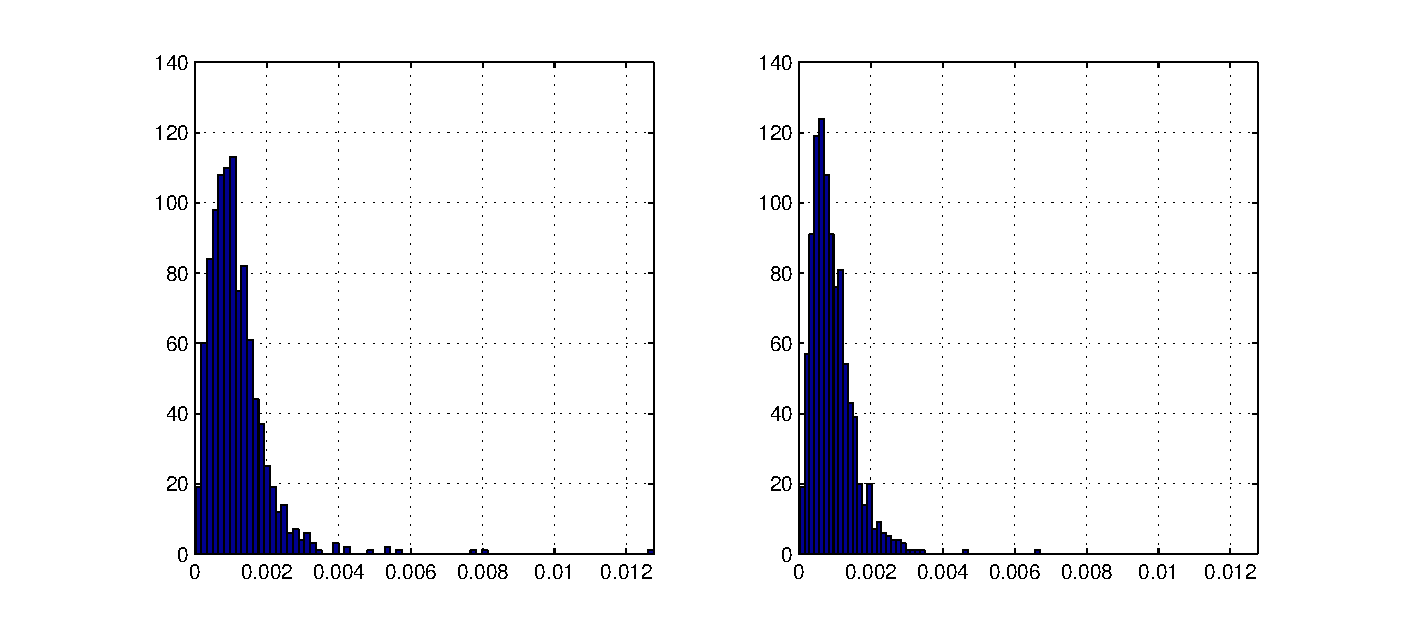
\includegraphics[width=1.2\textwidth]{figures/range_IRWLS/Noise03LeftBeckRightIrw}}
\caption{Histograms of the errors of the SR-LS (left) and IRWSR-LS (right) solutions, with standard deviation of noise $\protect\sigma = 10^{-3}$}
\label{fig:Noise03IRW}
\end{figure}

\begin{figure}%[t]
\centering
  \makebox[\textwidth][c]{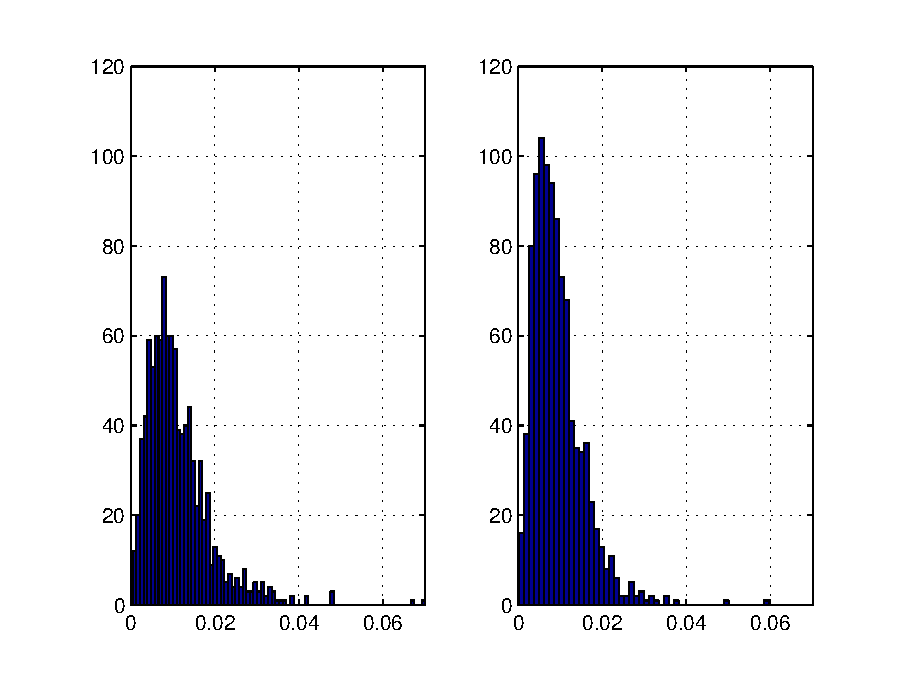
\includegraphics[width=1.1\textwidth,height=0.45\textheight]{figures/range_IRWLS/Noise02LeftBeckRightIrw}}
\caption{Histograms of the errors of the SR-LS (left) and IRWSR-LS (right) solutions,  with standard deviation of noise $\protect\sigma = 10^{-2}$}
\label{fig:Noise02IRW}
\end{figure}

\newpage

\begin{figure}[h]%[t]
\centering
  \makebox[\textwidth][c]{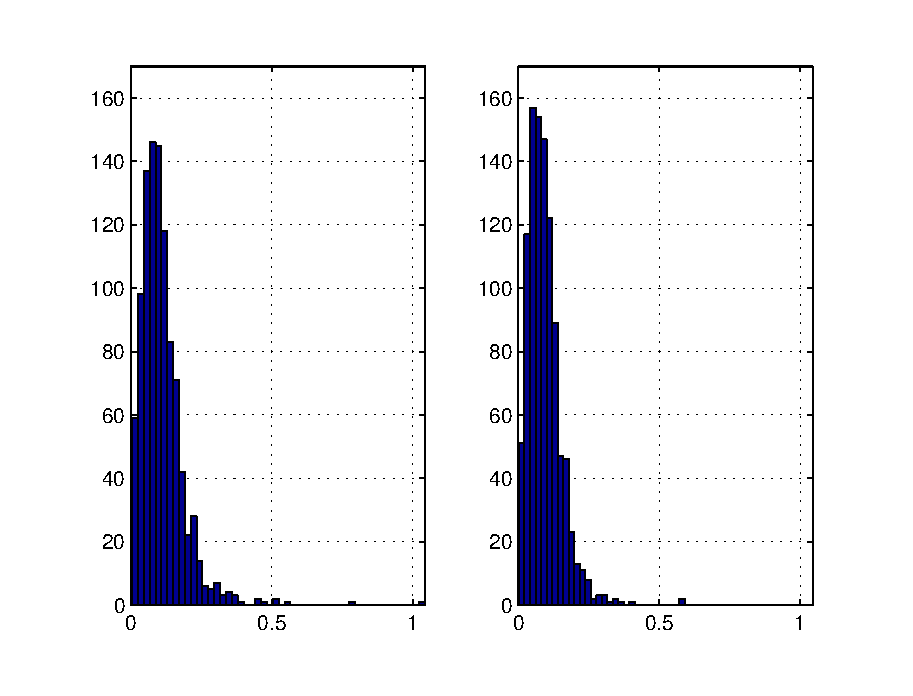
\includegraphics[width=1.1\textwidth,height=0.4\textheight]{figures/range_IRWLS/Noise01LeftBeckRightIrw}}
\caption{Histograms of the errors of the SR-LS (left) and IRWSR-LS (right) solutions,  with standard deviation of noise  $\protect\sigma = 10^{-1}$}
\label{fig:Noise01IRW}
\end{figure}

%\begin{figure}%[t]
%\centering
%  \makebox[\textwidth][c]{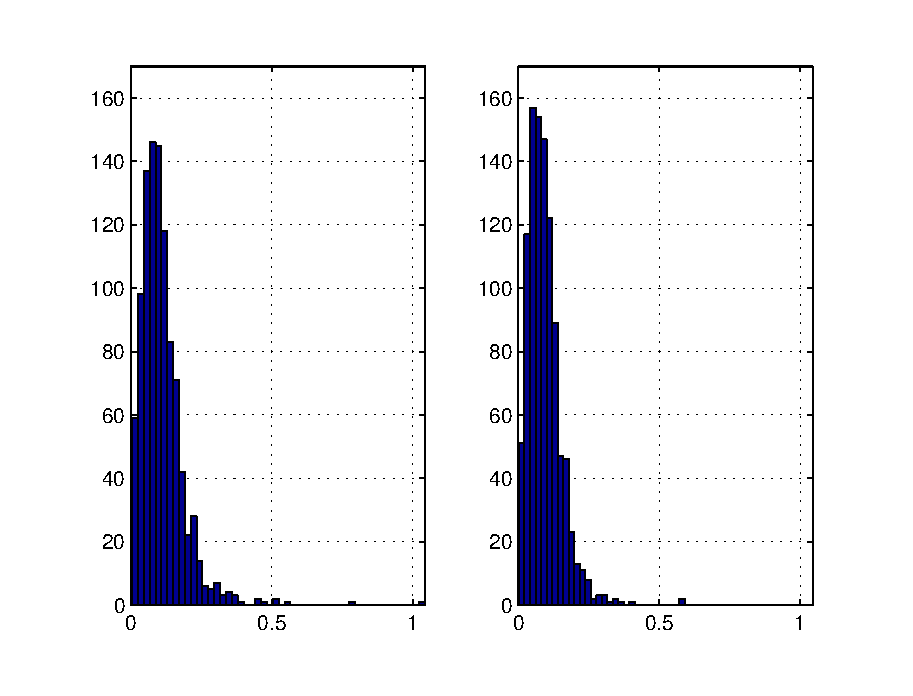
\includegraphics[width=1.1\textwidth,height=0.4\textheight]{figures/range_IRWLS/Noise01LeftBeckRightIrw}}
%\caption{Histograms of the errors of the SR-LS (left) and IRWSR-LS (right) solutions, noise $\protect\sigma = 1$}
%\label{fig:Noise00IRW}
%\end{figure}

\newpage

\section{Source Localization Using Range-Difference Measurements}%3
\subsection{Problem Formulation} %3.1

Another type of source localization problem that has attracted considerable attention is that of localizing a radiating source using range-difference measurements \cite{ StLi, BeckStLi}. In practice, range-difference measurements may be obtained from the time differences of arrival measured by an array of passive sensors. Time difference of arrival (TDOA) is a time-based positioning method based on the idea that the location of an active mobile unit (source of the signal)  can be determined by examining the difference in time at which the signal arrives at multiple reference points. 
Adopting this technique is useful in practical scenarios where synchronization between mobile units is not available \cite{GeoLoc}. A typical example can be found in 3G (WCDMA) and LTE networks where the observed time difference of arrival (O-TDOA) technique is used %Typical example of such setup includes the observed time difference of arrival (O-TDOA) technique used in 3G (WCDMA) and LTE networks 
to estimate the location of mobile units. We remark that in WCDMA networks, only the base stations are synchronized with each other, but mobile units are unsynchronized with base stations. 

Each TDOA measurement constrains the location of the signal source
%mobile device 
to be on a hyperboloid with a constant range-difference between the two reference points. Specifically a TDOA measurement between base stations $BS_i$ and $BS_0$ is given by 
\begin{equation}
\nonumber
t_{i0} = (t_i - t_x) - (t_0 - t_x) = t_i - t_0
\end{equation}
where $t_x$ is the clock time of the mobile unit, $t_i$ and $t_0$ are the time of arrival between the mobile unit and  stations $BS_i$ and $BS_0$ respectively. The above equation can be written in terms of distance (range-difference) through scaling 
\begin{equation}
\nonumber
r_{i} =(t_i - t_0)c = r_i - r_0 = \|\Ba_i - \Bx\| - \|\Ba_0 - \Bx\|, i = 1,\ldots,m
\end{equation}
where $c$ is the speed of signal propagation, $r_i$ is the distance from station $\Ba_i$ to source $\Bx$, $r_0$ is the distance from station $\Ba_0$ to source $\Bx$, and $\Ba_i \in R^n$ with $n = 2$ or $3$, contains coordinates of the $i$th base station.  Without loss of generality, the latter equation is valid with the assumption that the station $BS_0$ is placed at the origin of the coordinate system, i.e. $\Ba_0 = \BO$  and used as a \textit{reference} station \cite{GeoLoc}. 
%\cite{Liu} The idea of TDOA is to determine the relative position of the mobile transmitter by examining the difference in time at which the signal arrives at multiple measuring units, rather than the absolute arrival time. 
 
%obtained by comparing the signal as it is received at the $m+1$ sensors taken in pairs. 
%As usual, these sensors are denoted as $\{\Ba_0, \Ba_1,\ldots,\Ba_m\} \in R^n$ with $\Ba_0 = \BO$ be placed at the origin and used as a \textit{reference sensor}. The range-difference $r_i$ is defined as the difference between the distance from sensor $\Ba_i$ to source $\Bx$ and the distance from sensor $\Ba_0$ to source $\Bx$, namely %The range-difference measurements are obtained as

% \begin{equation} \label{eq:3.21}
% r_i=\|\Bx-\Ba_i\|-\|\Bx-\Ba_0\|=\|\Bx-\Ba_i\|-\|\Bx\|, i = 1,\ldots,m
% \end{equation}
The localization problem here is to estimate the location of a radiating source $\Bx$ given the locations of the $m+1$ sensors $\{\Ba_i, i = 0, 1, \ldots, m\}$ and noise-contaminated range-difference measurements $\{d_i, i = 1, 2, \ldots, m\}$ where 
\begin{equation} \label{eq:3.21}
d_i = r_i + \varepsilon_i = \|\Ba_i - \Bx\| - \|\Bx\| + \varepsilon_i, \mbox{ for } i = 1, 2, \ldots, m
\end{equation}
%based on measurements $d_i$'s. 
Therefore, the standard range-difference LS (RD-LS) problem is formulated as
 \begin{equation} \label{eq:3.22}
\Min_{\Bx \in R^n} F(\Bx)=\sum_{i=1}^m \left(d_i+\|\Bx\|-\|\Bx-\Ba_i\|\right)^2
 \end{equation}
 Unfortunately, problem (\ref{eq:3.22}) is nonconvex and finding the global solution of (\ref{eq:3.22}) turns out to be a very hard problem. Nonlinear least squares (NLLS) algorithm  \cite{{KimLeJe}} is widely used in TDOA localization systems for its performance. If  the range  measurement  errors  can  be  modeled  as  an  additive white  Gaussian  noise,  the  accuracy  of  NLLS solution approaches  the Cram$\acute{e}$r-Rao  lower  bound  (CRLB). However, NLLS is not guaranteed to converge  \cite{Chan}, \cite{KimLeJe} if the initial point is chosen far away from the actual source location. This becomes a more serious problem when the system coverage area is large since it becomes more difficult to secure an initial point that is close enough to the \textit{unknown} source location. The Scaling by  MAjorizing  a  COmplicated  Function  (SMACOF)  strategy proposed in \cite{SMAC} can also be applied for position estimation. Compared with NLLS, it is not sensitive to the choice of the initial point and the mean-square error is guaranteed to decrease at each iteration, however the algorithm  converges significantly slower.	
%{
%The proposed algorithm does not converge as fast as the NLLS algorithm, but it is not sensitive to the choice of
%the initial position, and the mean-square error is guaranteed to decrease at each iteration. More importantly, it does not
%require redundant receivers; when redundancy in the range measurements is unavailable, it can be used to provide the
%initial target position estimate for the NLLS algorithm. 
%Compared with  NLLS,  SMACOF  is  much  more  stable  but  it  converges significantly slower. When the number of anchors is large, both the  NLLS  and  SMACOF  methods  become  very  complex  to implement.  
%} 
%\textit{
%cite(fusion paper) Different aspects of positioning using passive ranging mea-
%surements have already been analyzed in the literature. Closed form solutions for hyperbolic positioning can be found for instance in [9]–[11]. Iterative algorithms for solving a nonlinear (weighted) least squares (N(W)LS) form another major group.
%The Gauss-Newton algorithm is studied in [12], constrained and non-constrained NLS solutions are discussed in [13], [14].
%The iterative approaches generally require good initialization to converge to the global optimum of the cost function and
%often many iterations. In order to avoid these issues, the solutions proposed in [15], [16] transform nonlinear equations into a set of linear ones, thus making real-time implementations possible. Factor graph-based methods carrying low-complex
%flags also attracted some attention [17], [18].
%......
%(cite NLOS mitigation)
%General nonlinear solutions are Maximum Likelihood (ML), Nonlinear Least Squares (NLS) or the Weighted Nonlinear Squares (WNLS) approach [5]. The WNLS solution
%requires minimization of a cost function, and performing ML estimation requires noise statistics. When the measurement
%noise n in (1) is zero-mean and Gaussian distributed with covariance matrix C n , ML scheme reduces to the WNLS solution.
%The ML approach requires a high complexity when grid search is performed, and therefore global solution may not
%be guaranteed, but in general its accuracy is the highest, especially when C n is also a function of subscriber position [6]. However, having a perfect error statistical characterization is
%difficult and others approaches are preferred. On the other hand, NLS does not require noise statistics but also involves
%the same issues as ML.
%} 
Reference \cite{BeckStLi} proposes a squared range-difference least squares (SRD-LS) approach to address this problem, which is summarized below.

 By writing (\ref{eq:3.21}) as $d_i+\|\Bx\|=\|\Bx-\Ba_i\|$ and squaring both sides, we obtain
  \begin{equation} \label{eq:3.23}
\left(d_i+\|\Bx\|\right)^2 = \|\Bx-\Ba_i\|^2
 \end{equation}
 which can be simplified to
  \begin{equation} \label{eq:3.24}
-2d_i\|\Bx\|-2\Ba_i^T\Bx=g_i, i=1,\ldots,m
 \end{equation}
 where $g_i=d_i^2-\|\Ba_i\|^2$. In practice (\ref{eq:3.24}) does not hold exactly due to measurement noise that contaminates the data $d_i$'s. In other words, if $d_i$'s in (\ref{eq:3.24}) are taken to be real-world data, then we only have
 \begin{equation} \label{eq:3.25}
-2d_i\|\Bx\|-2\Ba_i^T\Bx-g_i\approx 0, i=1,\ldots,m
 \end{equation}
 Reference \cite{BeckStLi} proposes a LS solution for the problem at hand by minimizing the sum of squared residues on the left side of (\ref{eq:3.25}), namely,
 \begin{equation}\label{eq:3.26}
\Min_{{\Bx} \in R^{n}} \sum_{i=1}^m \left(-2\Ba_i^T\Bx-2d_i\|\Bx\|-g_i\right)^2
\end{equation}
 By introducing new variable $\By=[\Bx^T \|\Bx\|]^T$ and noticing nonnegativity of the component $y_{n+1}$ problem (\ref{eq:3.26}) is converted to
 \begin{eqnarray}\label{eq:3.27}%40
\setcounter{abc}{1}
\Min_{\By\in R^{n+1}} \|\BB\By-\Bg\|^2 \\
\stepcounter{abc} \setcounter{equation}{27}
\mbox{subject to: } \By^T\BC\By = 0 \\
\stepcounter{abc} \setcounter{equation}{27}
y_{n+1}\geq 0
\end{eqnarray}
where 
\begin{equation}
\setcounter{abc}{0}
\Bg=\left(\begin{array}{cc}
g_1 \\
\vdots \\
g_m 
\end{array}\right), \;
\BB = \left(\begin{array}{cc}
    -2\Ba_1^T & -2d_1 \\
    \vdots & \vdots \\
    -2\Ba_m^T & -2d_m
    \end{array}\right), \;
\BC =  \left(\begin{array}{cc}
    \BI_n & \BO_{n \times 1} \\
    \BO_{1 \times n} & -1
    \end{array}\right)
\label{eq:3.28} %41
\end{equation} 
Because of the presence of the nonnegativity constraint in (\ref{eq:3.27}c), (\ref{eq:3.27}) is no longer a GTRS problem hence the technique used for the case of range measurements does not apply. Nevertheless reference \cite{BeckStLi} presents a rigorous argument which shows that the optimal solution of (\ref{eq:3.27}) either assumes the form of
 \begin{equation}
 \nonumber
 \tilde{\By}(\lambda)=\left(\BB^T\BB+\lambda\BC\right)^{-1}\BB^T\Bg
 \end{equation}
 where $\lambda$ solves
 \begin{equation}\label{eq:3.29}
 \tilde{\By}(\lambda)^T\BC\tilde{\By}(\lambda)=0
 \end{equation}
 and makes $\BB^T\BB+\lambda\BC$ positive definite, or is the vector among $\{\BO,$ $\tilde{\By}(\lambda_1),\ldots,\tilde{\By}(\lambda_p)\}$ that gives the smallest objective function in (\ref{eq:3.27}a), where $\{\lambda_i, i = 1,\ldots,p\}$ are all roots of (\ref{eq:3.29}) such that the $(n+1)$'th component of $\tilde{\By}(\lambda_i)$ is nonnegative and $\BB^T\BB+\lambda\BC$ has exactly one negative and $n$ positive eigenvalues. We shall refer the global solution of (\ref{eq:3.27}) to as the SRD-LS solution.

\subsection{Improved Solution Using Iterative Re-weighting} %3.2
%\subsubsection{Weighted squared range-difference based least squares solution}
\subsubsection{The Algorithm} %3.2.1

We now present a method for improved solutions over SRD-LS solutions. The method incorporates an iterative re-weighting procedure into the SRD-LS approach, hence it is in spirit similar to the IRWRS-LS approach described in Sec. \ref{chapter:irw}.1.2. We begin by considering the weighted squared range-difference least squares (WSRD-LS) problem
\begin{equation} \label{eq:3.30}
\Min_{{\Bx} \in R^n} \sum_{i=1}^m w_i\left(-2\Ba_i^T\Bx-2d_i\|\Bx\|-g_i\right)^2
\end{equation}
where weights $w_i$ for $i=1,\ldots,m$ are fixed nonnegative constants. The counterpart of (\ref{eq:3.27}) for the problem (\ref{eq:3.30}) is given by
\begin{eqnarray} \label{eq:3.31}
\setcounter{abc}{1}
\Min_{\By \in R^{n+1}} \|\BB_w\By - \Bg_w\| \\
\stepcounter{abc} \setcounter{equation}{31}
\mbox{subject to: } \By^T\BC\By = 0 \\
\stepcounter{abc} \setcounter{equation}{31}
y_{n+1}\geq 0
\end{eqnarray}
where $\Bg_w=\BGA\Bg$, $\BB_w=\BGA\BB$, $\BGA=\mbox{diag}\{\sqrt{w_1},\ldots,\sqrt{w_m}\}$, and $\Bg$, $\BB$ are defined in (2.28).
%, which will be referred to as the weighted SRD-LS (WSRD-LS) problem. 
 On comparing (\ref{eq:3.31}) with (\ref{eq:3.27}), it follows immediately that the global solver for problem (\ref{eq:3.27}) characterized by data set $\{\BB, \Bg, \BC\}$ can also be suited for solving problem (\ref{eq:3.31}) be used applying it to data set $\{\BB_w, \Bg_w, \BC\}$.
 
Concerning the assignment of weights $\{w_i, i=1,\ldots,w_m\}$, we recall (\ref{eq:3.23}), (\ref{eq:3.24}) and observe that the $i$th term of the objective function in (\ref{eq:3.30}) can be written as
\begin{equation} \label{w:srd}
\nonumber
\begin{aligned}
&w_i\left(-2d_i\|\Bx\|-2\Ba_i^T\Bx-g_i\right)^2 \\
=&w_i\left((d_i+\|\Bx\|)^2-\|\Bx-\Ba_i\|^2\right)^2 \\
=&w_i\left(d_i+\|\Bx\|+\|\Bx-\Ba_i\|\right)\left(d_i+\|\Bx\|-\|\Bx-\Ba_i\|\right)
\end{aligned}
\end{equation}
Clearly, the last expression above would become the $i$th term of the objective function in the RD-LS problem (\ref{eq:3.22}) if weights $w_i$ were set to
\begin{equation}
\nonumber
 \frac{1}{\left(d_i+\|\Bx\|+\|\Bx-\Ba_i\|\right)^2}
\end{equation} 
so that the first two factors are cancelled out. This suggests that a realizable weight assignment for performing practically the same cancellation can be made by means of iterative re-weighting for problems (\ref{eq:3.30}) and (\ref{eq:3.31}) where the weights in the $k$th iteration are assigned to
\begin{equation} \label{eq:3.32}
\setcounter{abc}{0}
w_i^{(k)}=\frac{1}{\left(d_i+\|\Bx_{k-1}\|+\|\Bx_{k-1}-\Ba_i\|\right)^2}, i=1,\ldots,m
\end{equation}

Based on the analysis above, a localization algorithm for range-difference measurements can be outlined as follows.

%\begin{table} \label{alg:rd-ls}
%\centering
%\caption{Iterative re-weighting least-squares method for source localization based on range-difference measurements.}
%\begin{tabular}{|l|l|} \hline
%\centering
%. & \textbf{Algorithm 3.2} \\ \hline
%%&&& \\ 
%\textbf{Input} &	Sensor locations $\{\Ba_i, i=0, 1,\ldots,m\}$ with $\Ba_0=\BO$, range-difference measurements $\{d_i, i = 1,\ldots,m\}$, maximum number of iterations $k_{max}$, convergence tolerance $\xi$.	
%\\ &\\ \hline
%\textbf{Output} & $\protect\Bx^*$ \\ & \\ \hline
%\textbf{Step 1} & Generate data set $\{\BB, \Bg, \BC\}$ as 
%$\Bg = \left(\begin{array}{c}
%    d_1^2 - \|\Ba_1\|^2 \\
%    \vdots \\
%    d_m^2 - \|\Ba_m\|^2
%    \end{array}\right), 
%\BB = \left(\begin{array}{cc}
%    -2\Ba_1^T & -2d_1 \\
%    \vdots & \vdots \\
%    -2\Ba_m^T & -2d_m
%    \end{array}\right),
%\BC =  \left(\begin{array}{cc}
%    \BI_n & \BO_{n \times 1} \\
%    \BO_{1 \times n} & -1
%   \end{array}\right).
%$
%Set $k=1$, $w_i^{(1)}=1$ for $i=1,\ldots,m$.
%\\ &\\ \hline
%\textbf{Step 2} &	 Set $\BGA_k=\mbox{diag}\left(\sqrt{w_1^{(k)}},\ldots,\sqrt{w_m^{(k)}}\right)$, $\BB_w=\BGA_k\BB$ and $\Bg_w=\BGA_k\Bg$.
%\\ &\\ \hline
%\textbf{Step 3} & Solve WSRD-LS problem
%$\Min_{\By \in R^{n+1}} \|\BB_w\By - \Bg_w\|$
%$ \mbox{subject to: } \By^T\BC\By = 0 $
%$y_{n+1}\geq 0$
%to obtain its global solution $\Bx_k$.	
%\\& \\ \hline
%\textbf{Step 4} & If $k=k_{max}$ or $\|\Bx_k-\Bx_{k-1}\|<\xi$, terminate and output $\Bx_k$ as the solution; otherwise, set $k=k+1$, update weights $\{w_i^{(k)}, i=1,\ldots,m\}$ as 
%$ w_i^{(k)}=\frac{1}{\left(d_i+\|\Bx_{k-1}\|+\|\Bx_{k-1}-\Ba_i\|\right)^2} $
%and repeat from Step 2.
%\\ %&&&&\\
%\hline
%\end{tabular}
%\end{table}

\phantom{m}
\framebox{%
\parbox{5.5in}{
\textbf{Algorithm 2} 

1) Input data: Sensor locations $\{\Ba_i, i=0, 1,\ldots,m\}$ with $\Ba_0=\BO$, range-difference measurements $\{d_i, i = 1,\ldots,m\}$, maximum number of iterations $k_{max}$ and convergence tolerance $\xi$.

2) Generate data set $\{\BB, \Bg, \BC\}$ as
\begin{equation} 
\nonumber
\setcounter{abc}{0}
\Bg = \left(\begin{array}{c}
    d_1^2 - \|\Ba_1\|^2 \\
    \vdots \\
    d_m^2 - \|\Ba_m\|^2
    \end{array}\right),
\BB = \left(\begin{array}{cc}
    -2\Ba_1^T & -2d_1 \\
    \vdots & \vdots \\
    -2\Ba_m^T & -2d_m
    \end{array}\right),
\BC =  \left(\begin{array}{cc}
    \BI_n & \BO_{n \times 1} \\
    \BO_{1 \times n} & -1
    \end{array}\right).
\end{equation}
Set $k=1$, $w_i^{(1)}=1$ for $i=1,\ldots,m$.

3) Set $\BGA_k=\mbox{diag}\left(\sqrt{w_1^{(k)}},\ldots,\sqrt{w_m^{(k)}}\right)$, $\BB_w=\BGA_k\BB$ and $\Bg_w=\BGA_k\Bg$.

4) Solve WSRD-LS problem
\begin{eqnarray}
\nonumber
\Min_{\By \in R^{n+1}} \|\BB_w\By - \Bg_w\| \\
\nonumber
\mbox{subject to: } \By^T\BC\By = 0 \\
\nonumber
y_{n+1}\geq 0
\end{eqnarray}
to obtain its global solution $\Bx_k$.

5) If $k=k_{max}$ or $\|\Bx_k-\Bx_{k-1}\|<\xi$, terminate and output $\Bx_k$ as the solution; otherwise, set $k=k+1$, update weights $\{w_i^{(k)}, i=1,\ldots,m\}$ as 
\begin{equation}
\nonumber
\setcounter{abc}{0}
w_i^{(k)}=\frac{1}{\left(d_i+\|\Bx_{k-1}\|+\|\Bx_{k-1}-\Ba_i\|\right)^2}
\end{equation}
and repeat from Step 3).
}
} \label{alg:rd-ls}

%\phantom{m}

It is evident that the complexity of the algorithm is practically equal to the complexity of the WSRD-LS solver involved in Step 4 times the number of iterations, $k$, which is typically in the range of 3 to 6. We shall call the solutions obtained from Algorithm 2 IRWSRD-LS solutions. Technical details with regard to solving problem (\ref{eq:3.31}) can be found in Appendix 1.


\subsubsection{A variant of Algorithm 2}

Like the case of range measurements, once the IRWSRD-LS solution is obtained by applying Algorithm 2, which is expected to be within a small vicinity of the true global solution of the RD-LS problem (\ref{eq:3.22}), the gap can be closed by running a good local method that takes the IRWSRD-LS solution as an initial point. Again, the Newton method is chosen for fast convergence, low complexity due to the extremely low dimension $n$, and the availability of closed-form formulas to compute the gradient and Hessian of $F(\Bx)$ in (\ref{eq:3.22}).

Assuming $\Bx\neq\Ba_i$ for $i = 0, 1,\ldots, m$, the gradient and Hessian of $F(\Bx)$ is found to be
\begin{equation}
\nonumber
\Bg(\Bx)=\sum_{i=1}^m c_i\left(\Bq_i - \tilde(\Bx)\right)
\end{equation}
and
\begin{equation}
\nonumber
\BH(\Bx)=\sum_{i=1}^m \left[(\Bq_i-\tilde(\Bx))(\Bq_i-\tilde(\Bx))^T+c_i(\BQ_{1i}+\BQ_2)\right]
\end{equation}
respectively, where
\begin{equation}
\nonumber
c_i=\|\Bx-\Ba_i\|-\|\Bx\|, \Bq_i=\frac{\Bx-\Ba_i}{\|\Bx-\Ba_i\|}, \tilde{\Bx}=\frac{\Bx}{\|\Bx\|}
\end{equation}
and
\begin{equation}
\nonumber
\BQ_{1i}=\frac{1}{\|\Bx-\Ba_i\|}\left(\BI-\Bq_i\Bq^T\right), \BQ_2=\frac{1}{\|\Bx\|}\left(\BI-\tilde{\Bx}\tilde{\Bx}^T\right)
\end{equation}
To ensure the positive definiteness of Hessian, eigen-decomposition of $\BH(\Bx)$, namely,
\begin{equation}
\nonumber
\BH(\Bx)=\BU\BLA\BU^T
\end{equation}
is performed, where $\BU$ is orthogonal and $\BLA=\mbox{diag}(\lambda_1,$ $\ldots,\lambda_n)$ with $\{\lambda_i, i=1,\ldots,n\}$ being the eigenvalues of $\BH(\Bx)$. Let $\lambda_{min}$ be the smallest eigenvalue of $\BH(\Bx)$. If $\lambda_{min}$, then $\BH(\Bx)$ is positive definite and the Newton algorithm is carried out without modification; if $\lambda_{min}\leq0$, then the algorithm uses a slightly modified Hessian given by
\begin{equation}
\nonumber
\tilde{\BH}(\Bx)=\BU\tilde{\BLA}\BU^T
\end{equation}
where $\tilde{\BLA}=\mbox{diag}\left(\tilde{\lambda}_1,\ldots,\tilde{\lambda}_n\right)$ with
\begin{equation}
\nonumber
\tilde{\lambda}_i=\left\{\begin{array} {lll}
    \lambda_i & \mbox{if } \lambda_i>0 & \\
    \delta &  \mbox{if } \lambda_i\leq0 & i=1,\ldots,m \end{array} \right.
\end{equation}
and $\delta$ a small positive constant. Obviously, $\tilde{\BH}(\Bx)$ is guaranteed to be positive definite. In what follows, solutions obtained by the proposed two-step method are called \textit{hybrid} IRWSRD-LS solutions.

\subsection{Numerical Results}

Performance of the proposed algorithms was evaluated and compared with the method of  \cite{BeckStLi} by Monte Carlo simulations with a set-up similar to that of \cite{BeckStLi}. SRD-LS solutions were used as performance benchmarks for Algorithm 2 and its variant. In both cases the system consisted of $m = 11$ sensors $\{\Ba_i, \ i=1, 2,\ldots, 10\}$ with $\Ba_0 = \BO$ and other ten sensors placed randomly placed in the planar region $[-15;15]\times[-15;15]$, and a radiating source $\Bx_s$, located randomly in the region $[-10;10]\times[-10;10]$. Coordinates of the source and sensors were generated for each dimension following a uniform distribution. The range-difference measurements used to form  matrix $\BB$ in Step 2 of the Algorithm 2 were calculated as noise-contaminated range-difference measurements $d_i$ in (\ref{eq:3.21}). Measurement noise $\{\varepsilon_i, \ i = 1,\ldots, m\}$ was modelled as i.i.d. random variables with zero mean and variance $\sigma^2$, with $\sigma$ being one of five possible levels $\{10^{-4}, 10^{-3}, 10^{-2}, 10^{-1}, 1\}$. Step 4 of Algorithm 2 was carried out using the SRD-LS algorithm in \cite{BeckStLi}.  Accuracy of source location estimation was evaluated in terms of mean squared error in the form $\mbox{MSE} = E\{\|\Bx^*-\Bx_s\|\}$ where $\Bx_s$ denotes the exact source location and $\Bx^*$ is its estimation obtained by SRD-LS, IRWSRD-LS and \textit{hybrid} IRWSRD-LS methods, respectively. Table \ref{tab:3} provides comparisons of these methods with SRD-LS, where each entry was averaged MSE over 1,000 Monte Carlo runs of the method. For the columns representing performance of the IRWSDR-LS and \textit{hybrid} IRWSDR-LS methods each table entry lists their MSE and relative improvement over SRD-LS solutions in percentage, in the format of MSE ($\%$ Improvement). Again, the IRWSRD-LS solutions offer considerable improvement over SRD-LS solutions. Further analysis of the data that was used to generate Table \ref{tab:3} illustrates the advantage of the IRWSR-LS (hybrid IRWSR-LS) solution over the SR-LS. 
Each entry in Table \ref{tab:4} is a standard deviation of the squared  estimation errors  aggregated over the  same 1,000 Monte Carlo runs described above in Table \ref{tab:3} (where the MSE of the position estimation are shown). The results summarised in Table \ref{tab:4} suggest that, again, IRWSR-LS and hybrid IRWSR-LS outperform SR-LS. 
%\setlength{\textfloatsep}{5pt}
\setlength{\intextsep}{5pt}

\begin{table}[h]
\centering
\caption{MSE of position estimation for SRD-LS, IRWSRD-LS and \textit{hybrid} IRWSRD-LS methods}
\phantom{m}
\begin{tabular}{|c|c|c|c|} \hline
\centering
$\sigma$ & SR - LS & IRWSR-LS (Im.,\%) & \textit{hybrid} IRWSR-LS (Im.,\%) \\ \hline
%&&& \\
1e-04&  1.38301598e-08 & 8.22705918e-09 (40) &  8.22705918e-09 (40) \\ &&&\\ 
1e-03&	1.60398717e-06 & 1.03880406e-06 (35)&  1.038804061e-06 (35) \\ &&&\\
1e-02&	1.11632818e-04 & 6.67785604e-05 (40)&  6.67265316e-05 (40)  \\ &&&\\
1e-01&	1.20947651e-02 & 7.20891487e-03 (40)&  7.07178346e-03 (41) 	 \\ &&&\\
1e+0&	1.57050323e+00 & 9.70756420e-01 (40)&  7.86289933e-01 (48)  \\ %&&&&\\
\hline
\end{tabular}
\label{tab:3}
%\end{table}
%\begin{table}[h]
\centering
\caption{Standard deviation of the squared estimation error for SRD-LS, IRWSRD-LS and \textit{hybrid} IRWSRD-LS methods}
\phantom{m}
\begin{tabular}{|c|c|c|c|} \hline
$\sigma$ & SR - LS & IRWSR-LS & \textit{hybrid} IRWSR-LS \\ \hline
%&&& \\ 
1e-04&  4.5624e-08 &   2.2446e-08 &  2.2446e-08\\ &&&\\
1e-03&	3.9506e-06 &   3.1610e-06 &  3.1610e-06\\ &&&\\
1e-02&	2.2710e-04 &   1.2812e-04 &  1.2812e-04\\ &&&\\
1e-01&	3.0108e-02 &   1.8891e-02 &  1.8891e-02\\ &&&\\
1e+0&	4.5781e+00 &   3.0597e+00 &  3.0597e+00\\ %&&&&\\
\hline
\end{tabular}
\label{tab:4}
\end{table}

Figures \ref{fig:Noise00IRDW} to \ref{fig:Noise04IRDW} represent the histograms of the location estimation errors $\|\Bx^* - \Bx_s\|$ of the SR-LS solution (left images) and IRWSR-LS (right images) for all four noise levels with $\sigma$ being one of $\{10^{-3}, 10^{-2}, 10^{-1}, 1\}$, where $\Bx^*$ denotes the estimated location and $\Bx_s$ is the exact location of the source. Histograms that correspond to the results obtained by IRWSRD-LS are shifted closer towards $0$ than those obtained by SR-LS, have smaller variance, and in most cases solutions obtained by IRWSRD-LS have fewer outliers.

%\phantom{m}
%1e-4		1.383015982829804e-08     8.227059183670454e-09     8.227059183670454e-09
%1e-3		1.603987166725750e-06     1.038804061206498e-06     1.038804061206498e-06
%1e-2		1.116328181257473e-04     6.677856041622635e-05     6.672653163830277e-05
%1e-1 	1.209476513987653e-02     7.208914870970552e-03     7.071783455050626e-03
%1       1.513403231137539e+00     9.007964195574626e-01     7.862899335956174e-01

%1e-04& 1.3830e-08  & 8.2271e-09 (40) &  8.2270e-09 (40) \\ &&&\\ 
%1e-03&	1.3063e-06  & 8.2828e-07 (37)&  8.2827e-07 (37) \\ &&&\\
%1e-02&	1.1163e-04  & 6.6779e-05 (40)&  6.6779e-05 (40)  \\ &&&\\
%1e-01&	1.2095e-02  & 7.2089e-03 (40)&  7.2089e-03 (40) 	 \\ &&&\\
%1e+0&	1.5705e+00  & 9.7075e-01 (38)&  9.7075e-01 (38)  \\ %&&&&\\

%\setlength{\textfloatsep}{3pt}
%\setlength{\intextsep}{3pt}
%\setlength{\floatsep}{3pt}
%\setlength{\textfloatsep}{0.9\baselineskip plus 0.2\baselineskip minus 0.2\baselineskip}


\begin{figure}
\centering
  %\makebox[\textwidth][c]{
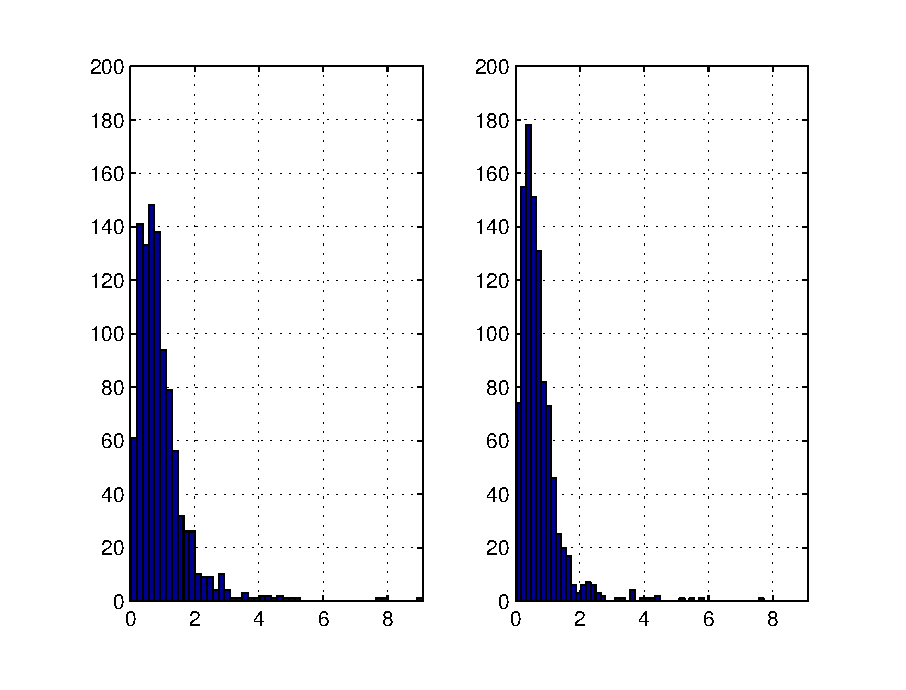
\includegraphics[width=1\textwidth,height=0.4\textheight]{figures/range_dif_IRWLS/Noise00LeftBeckRightRD}%}
\caption{Histograms of the errors of the SR-LS (left) and IRWSR-LS (right) solutions, with standard deviation of noise $\protect\sigma = 1$}
\label{fig:Noise00IRDW}
%\end{figure}
%\begin{figure}%[h]
\centering
  %\makebox[\textwidth][c]{
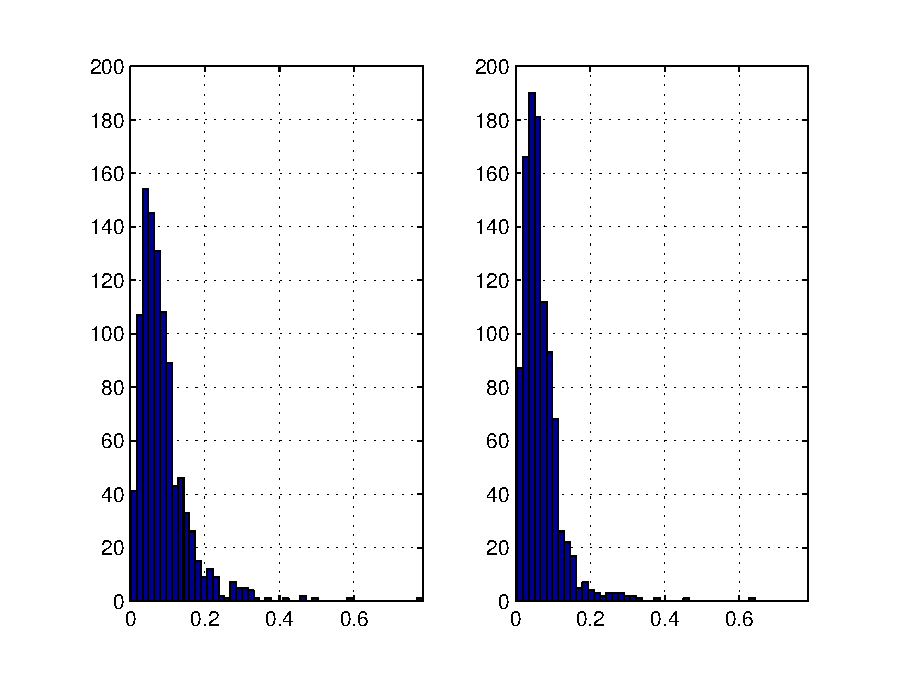
\includegraphics[width=1\textwidth,height=0.4\textheight]{figures/range_dif_IRWLS/Noise01LeftBeckRightRD}%}
\caption{Histograms of the errors of the SR-LS (left) and IRWSR-LS (right) solutions, with standard deviation of noise  $\protect\sigma = 10^{-1}$}
\label{fig:Noise01IRDW}
\end{figure}

%\newpage

\begin{figure}
\centering
 %\makebox[\textwidth][c]{
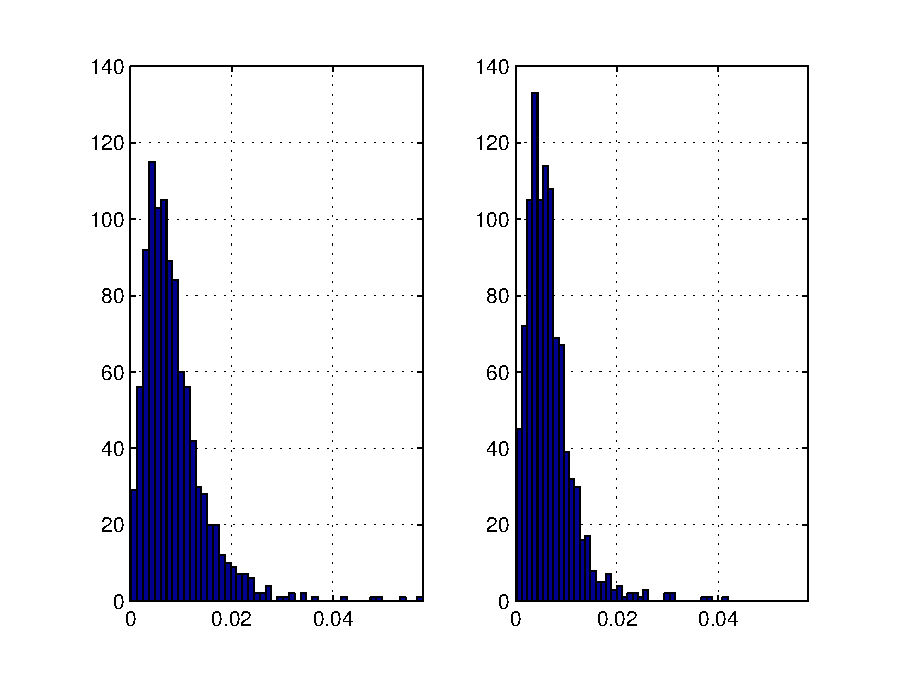
\includegraphics[width=1\textwidth,height=0.42\textheight]{figures/range_dif_IRWLS/Noise02LeftBeckRightRD}%}
\caption{Histograms of the errors of the SR-LS (left) and IRWSR-LS (right) solutions, with standard deviation of noise  $\protect\sigma = 10^{-2}$}
\label{fig:Noise02IRDW}
%\end{figure}
%\begin{figure}%[b]
\centering
%\makebox[\textwidth][c]{
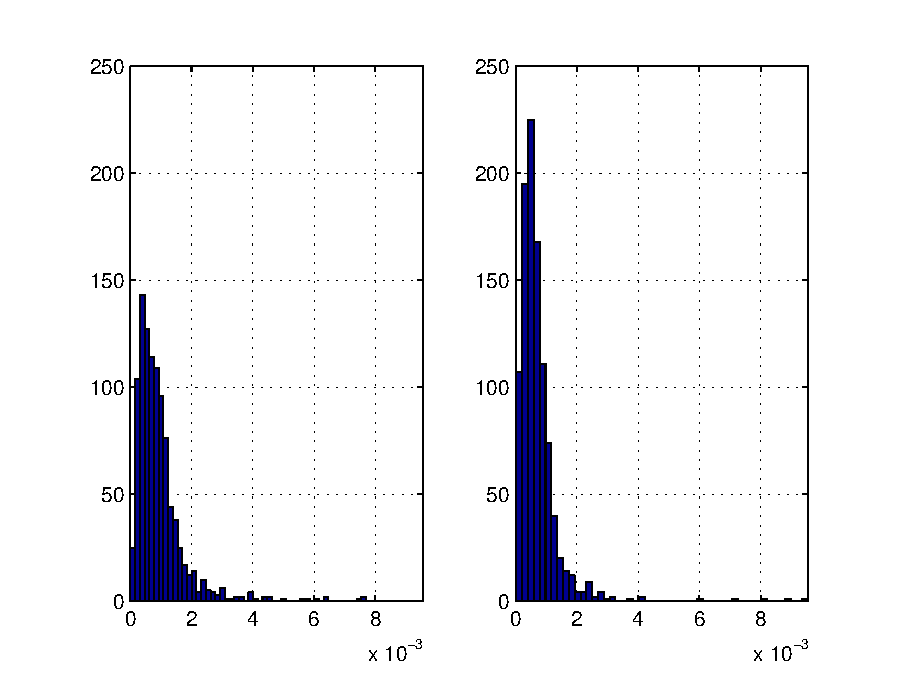
\includegraphics[width=1\textwidth,height=0.42\textheight]{figures/range_dif_IRWLS/Noise03LeftBeckRightRD}%}
\caption{Histograms of the errors of the SR-LS (left) and IRWSR-LS (right) solutions, with standard deviation of noise  $\protect\sigma = 10^{-3}$}
\label{fig:Noise03IRDW}
\end{figure}

\newpage

\begin{figure}[h]
\centering
 %\makebox[\textwidth][c]{
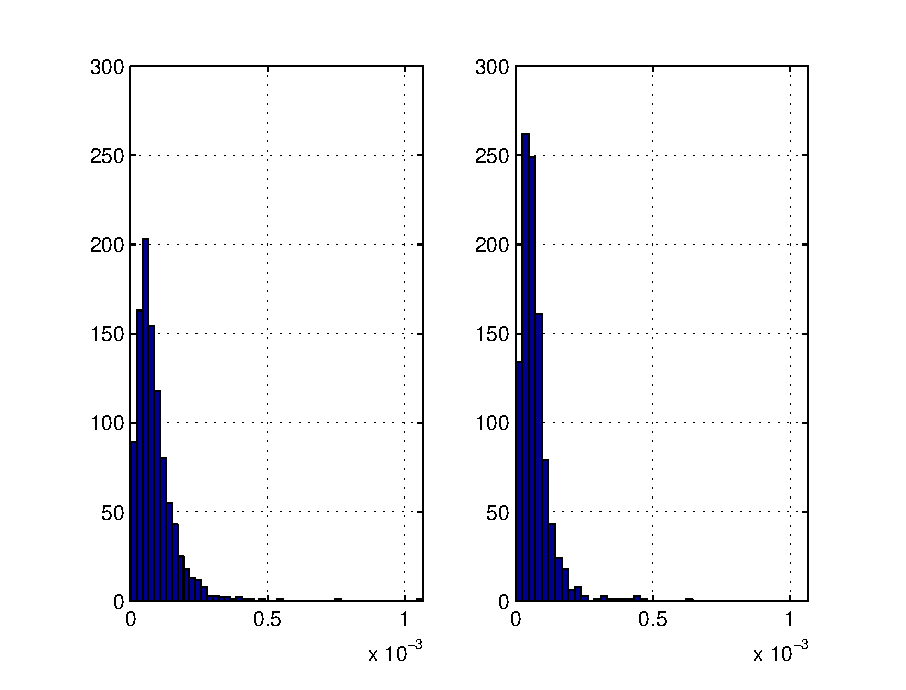
\includegraphics[width=1\textwidth,height=0.42\textheight]{figures/range_dif_IRWLS/Noise04LeftBeckRightRD}%}
\caption{Histograms of the errors of the SR-LS (left) and IRWSR-LS (right) solutions, with standard deviation of noise  $\protect\sigma = 10^{-4}$}
\label{fig:Noise04IRDW}
\end{figure}

%\newpage

\section{Extensions}


Methods developed in this chapter for localization based on range measurements can also be adopted to solve the problem of single sourse localization using energy measurements \cite{StLi}. 
% \cite{LiHu,ShengHu,Saric} \cite{LuWuYan}
%The energy, acoustic or RF, of the signal received by the sensor is inversely proportional to the distance between sensor and the radiating source (\cite{LiHu,ShengHu,Saric}).
%The localization based on the received signal strength uses the property that sound energy attenuates with the square of the distance from the source \cite{Saric}.
Energy-based source localization, advocated in \cite{LiHu}, \cite{Saric}, is motivated by the simple observation that the sound intensity received by a listener decreases when the distance between the sound source and the listener increases. By modeling the relation between sound intensity (energy) and distance from the sound source, one may estimate the source location using multiple energy readings at different known sensor locations. It is known that when the sound is propagating through the air, the acoustic energy emitted omnidirectionally from a sound source will attenuate at a rate that is inversely proportional to the square of the distance \cite{LiHu}. Using this fact and some simple manipulations, it is possible to obtain an equation in the vector of unknow source location $\Bx$ that is somewhat similar to (\ref{eq:3.9}). The rest of the section provides technical details of this reformulation. 

%(from \cite{StLi}) "The source localization problem from range measurements is related to the problem of source localization from energy measurements \cite{LiHu,ShengHu,Saric}.
%The energy measurement based source localization approach, advocated in \cite{LiHu}, \cite{Saric} is based on the fact that the energy of the signal received by the $i$th sensor over a (relatively small) time interval is inversely proportional to $\| \Bx - \Ba_i \|$, for $i = 1, 2, \ldots,m$. 

%Using this fact and some simple manipulations (see, e.g., \cite{LiHu} for details), it is possible to obtain an equation in the unknown vector x that is somewhat similar to (2), namely:....."

%This section provides an example of ...
%In this section, a reformulation of the maximum liklihood source localization using acoustic energy meausrements is offered.
%Acoustic energy attenuation model presented here is based on assumptions of \cite{LiHu} and \cite{Saric} (or please refer for details). Only single sourse localization is investigated in this section.

%\subsection{Acoustic Energy Attenuation Model} %and Parameter Estimator}


Let $m$ be a number of acoustic sensors involved. For consistency of notation, let $\Ba_i$ denote the known location of the sensor $i$ in space $R^n$ with $n = 2$ or $3$. Each sensor measures the acoustic intensity radiated by a source $\Bx\in R^n$ over a time period $T = \frac{M}{f_s}$, where $M$ is the number of sample points used for estimating the acoustic enery and $f_s$ is the sampling frequency. % (\textbf{OR} Received signal is an acoustic pulse $M$-samples wide.)
 Acoustic energy received by sensor $i$ over a time period $T$ can be represented as
\begin{equation} \label{eq:3.33}
r_i = g_i \frac{S}{\|\Bx - \Ba_i\|^\alpha} + \varepsilon_i
\end{equation}
where $\|\Bx - \Ba_i\|$ is the Euclidean distance between the $i$th sensor and the source, and $g_i$ is a scaling factor that takes into account $i$th sensor gain. It is asssumed that the gain of individual sensors is either known, i.e. obtained at the sensor callibration stage, or is same for all sensors. In (\ref{eq:3.33}) $S$ is the unknown acoustic energy measured 1 unit distance away from the source, $\alpha$ is the energy decay factor %(pathloss exponent) 
and is usually assumed to have a value 2 \cite{LiHu}, and $\varepsilon_i$ denotes the square of the background noise affecting the measurement of sensor $i$. If the number of sample points $M$ used for estimating the acoustic energy  is large, the error $\varepsilon_i$ can be approximated well as a normal distribution with positive mean $\mu_i$ and variance $\sigma_i^2$ %/ It is assumed to be a wide-sense stationary Gaussian random process \cite{LiuHuPan} / 
%, namely, $\varepsilon_i \sim N(\mu_i, \sigma_i^2)$ with a positive mean value $\mu_i$ that is no less than the standard deviation $\sigma_i$ that can be estimated empirically from data samples 
\cite{LiHu}, \cite{ShengHu}. More details on derivation and assumptions of this model can be found in %For justification and validity of this energy attenuation model, please see 
\cite{LiHu} - \cite{Saric}, \cite{LiuHuPan} and the references therein. %\cite{ShengHu},


References \cite{LiHu,ShengHu} argue that the maximum likelihood estimation of unknown parameters $\Btheta = [\Bx^T S]^T$ can be obtained by solving the minimization problem
\begin{equation} \label{eq:3.34}
\Min_\theta \quad \ell(\Btheta) = \|\BZ - S\BH\|
\end{equation}
where 
\begin{equation}
\nonumber
\BH = \left( \begin{array}{c}
\frac{g_1}{\sigma_1\|\boldsymbol{x} - \boldsymbol{a}_1 \|^2} \\
\frac{g_2}{\sigma_2\|\boldsymbol{x} - \boldsymbol{a}_2 \|^2} \\
\vdots \\
\frac{g_m}{\sigma_m\|\boldsymbol{x} - \boldsymbol{a}_m \|^2} \\
\end{array}
\right) , \;
\nonumber
\BZ = \left( \begin{array}{c}
\frac{y_1 - \mu_1}{\sigma_1} \\
\frac{y_2 - \mu_2}{\sigma_2} \\
\vdots \\
\frac{y_m - \mu_m}{\sigma_m} \\
\end{array}
\right)
\end{equation}
and $\BZ$ are (estimated) normalized energy measurements for the case of the single radiating source. We remark that $\mu_i$ and $\sigma_i$ in (\ref{eq:3.34}) are assumed to be known. 


\subsection{Reformulation}

There are two things to note about (\ref{eq:3.34}). First, (\ref{eq:3.34}) involves a \textit{nonlinear} least square objective function because the vector $\BH$ is a nonlinear function of the $n$  unknown source coordinates, where $n$ is the dimention of the location coordinates. Second, there are $m$ sensors reporting the acousting readings and there are a total of $n + 1$ unknowns with  $n + 1 \leq m$, including the unknown acoustic energy $S$ radiated from the source. To eliminate the unknown source energy $S$ from formultion, reference \cite{ShengHu}  propose first to compute the ratio $k_{ij}$ of the calibrated energy readings from $i$th and $j$th sensor as
\begin{equation} \label{eq:3.35}
k_{ij} = \left( \frac{z_i / g_i}{z_j / g_j} \right)^{-1/\alpha} = \frac{\|\Bx - \Ba_i\|}{\|\Bx - \Ba_j\|}
\end{equation}
for $i = 1, 2, \ldots, m-1$, and $j = i+1, \ldots, m$. For the case $0 < k_{ij} \neq 1$ all possible source coordinates $\Bx$ that form a solution to (\ref{eq:3.35}) reside on an $n$-dimensional hyper-sphere described by the equation:
\begin{equation} \label{eq:3.36}
\| \Bx - \Bc \|^2 = \rho_{ij}^2
\end{equation}
where the center $\Bc_{ij}$ and the radius $\rho_{ij}$ of the hyper-sphere associated with the sensors $i$ and $j$  are given by
\begin{equation} \label{eq:3.37}
\Bc_{ij} = \frac{\Ba_i - k_{ij}^2\cdot\Ba_j}{1-k_{ij}^2}, \;
 \rho_{ij} = \frac{k_{ij}\|\Ba_i - \Ba_j\|}{1-k_{ij}^2}
\end{equation}
For the case when $k_{ij} \rightarrow 1$, the possible source locations $\Bx$ reside on the hyperplane between sensors $\Ba_i$ and $\Ba_j$, i.e.:
\begin{equation}
\nonumber
\Bx^T \Bgamma_{ij} = \tau_{ij}
\end{equation}
where $\Bgamma_{ij} = \Ba_i - \Ba_j$ and $\tau_{ij} = (\|\Ba_i\|^2 - \|\Ba_j\|^2) / 2$. 

Let $I_1$ and $I_2$ be two index sets such that $0 < k_{ij} \neq 1$ for all $\{i, j \} \in I_1$ and $k_{ij} = 1$ for all $\{i, j\} \in I_2$ with $1 \leq i \leq m-1, i+1 \leq j \leq m $   and $I_1 \cap I_2 = \emptyset$.
Let $L_1$ and $L_2$ denote the number of elements in sets $I_1$ and $I_2$ respectively (number of hyperspheres and hyperplanes) and $L_1 + L_2 = m(m-1)/2$. Then the unknown location of the source can be found via minimization of the following criterion which is equivalent to (\ref{eq:3.34}) \cite{ShengHu}
\begin{equation} \label{eq:3.38}
%\Min \sum_{i,j \in I_1}^{} \left(\ \|\Bx - \Bc_{ij}\|^2 - \rho_{ij}^2\right)^2 + \sum_{i,j \in I_2}^{} \left( \Bx^T \Bgamma_{ij}  - \tau_{ij}\right)^2
\Min_{\Bx} \sum_{l_1 = 1}^{L_1} \left(\ \|\Bx - \Bc_{l_1}\|^2 - \rho_{l_1}^2\right)^2 + \sum_{l_2 = 1}^{L_2} \left( \Bx^T \Bgamma_{l_2}  - \tau_{l_2}\right)^2
\end{equation}
For the brevity of notation, the double indexes $ij$ were replaced by single indexes $l_1$ and $l_2$.  After some simple manupilations and necessary variable changes, (\ref{eq:3.38}) can be converted to the following constrained problem which is similar to (\ref{eq:3.10})
\begin{eqnarray} \label{eq:3.39}
\setcounter{abc}{1}
\Min_{{\By} \in R^{n+1}} \|\BA\By-\Bb\|^2 \qquad\\
\stepcounter{abc} \setcounter{equation}{39} \mbox{subject to: \ }
\By^T\BD\By + 2\Bf^T\By = 0
\end{eqnarray}
where
\begin{equation} \label{eq:3.40}
\setcounter{abc}{0}
\By = \left( \begin{array}{c}
 \Bx \\
 \|\Bx\|^2 
 \end{array}\right), \;
\BA=\left(\begin{array}{c}
    \BA_1 \\
    \BA_2
    \end{array} \right), \;
\Bb=\left(\begin{array}{c}
    \Bb_1 \\
    \Bb_2
    \end{array} \right)
\end{equation}
\begin{equation}% \label{eq:3.12}
\nonumber
\BD=\left(\begin{array}{cc}
    \BI\!_{n\times n} & \BO_{n\times 1} \\
    \BO_{1\times n} & 0
    \end{array} \right), \;
\Bf=\left(\begin{array}{c}\BO \\ -0.5 \end{array} \right)
\end{equation}
and submatrices of $\BA$ and elements of $\Bb$ are formed as follows:
\begin{equation} \label{eq:3.41}
\setcounter{abc}{0}
\setcounter{equation}{41}
\BA_1 = \left(\begin{array}{cc}
    -2\Bc_1^T & 1 \\
    \vdots  & \vdots \\
    -2\Ba_{L_1}^T & 1
    \end{array} \right), \;
\Bb_1 = \left(\begin{array}{c}
    \rho_1^2-\|\Bc_1\|^2 \\
    \vdots \\
    \rho_{L_1}^2-\|\Bc_{L_1}\|^2
    \end{array} \right)
\end{equation}
\begin{equation}
\nonumber
\BA_2 = \left(\begin{array}{cc}
    \gamma_1^T & 0 \\
    \vdots  & \vdots \\
    \gamma_{L_2}^T & 0
    \end{array} \right), \;
\Bb_2 = \left(\begin{array}{c}
    \tau_1 \\
    \vdots \\
    \tau_{L_2}
    \end{array} \right)
\end{equation}
The unconstrained problem in (\ref{eq:3.38}), due to mathematical analogy with (\ref{eq:3.9}), can be solved using Algorithm 1 developed in Section 3.1.